\documentclass
[12pt,
a4paper,
]{report}

\usepackage{ucs}
\usepackage[utf8x]{inputenc}
\usepackage[OT1]{fontenc}
\usepackage[frenchb]{babel}
\usepackage{lmodern}

\usepackage{makeidx}
\makeindex

\usepackage[rflt]{floatflt}
\usepackage{pdfpages}
\usepackage{url}
\usepackage{hyperref}
\hypersetup
{
	% bookmarks=true,
	unicode=true,
    pdfauthor={Riadh Habbachi},
    pdfsubject={Rapport de project de fin d'etudes},
    pdftitle={Mémoire de Projet de Fin d’Etudes-Développement d'une application Android pour médecins.},
    pdfkeywords={ENIG, Tunav, Stage, Stage ingenieur, project de fin d'etudes, LaTeX, PDF, hyperlinks}
}

\usepackage{color}
\usepackage{xcolor}
\usepackage{listings}
\lstloadlanguages{
	XML,
	Java
}
\lstset{
	basicstyle=\footnotesize\ttfamily,
	breaklines=true
}
\usepackage{caption}
\DeclareCaptionFont{white}{\color{white}}
\DeclareCaptionFormat{listing}{\colorbox{gray}{\parbox{\textwidth}{#1#2#3}}}
\captionsetup[lstlisting]{format=listing,labelfont=white,textfont=white}

\usepackage[stable]{footmisc}

\usepackage{array}
% \usepackage{tablefootnote}

\usepackage{graphicx}
\usepackage{float}
\usepackage{wrapfig}
\usepackage{subfig}

\newcommand{\en}[1]{\textit{#1}}
\newcommand{\android}{Android\texttrademark}
\newcommand{\dev}[1]{\textit{#1}}
\newcommand{\pct}{PowerChart Touch\texttrademark}
\newcommand{\tm}[1]{\textbf{#1}\texttrademark}
\newcommand{\cmd}[1]{\textbf{#1}}

\graphicspath{{../res/}}

\usepackage[nomain, toc, acronym]{glossaries}
%!TEX root = report.tex

%from documentation
%\newacronym[⟨key-val list⟩]{⟨label ⟩}{⟨abbrv ⟩}{⟨long⟩}
%above is short version of this
% \newglossaryentry{⟨label ⟩}{type=\acronymtype,
% name={⟨abbrv ⟩},
% description={⟨long⟩},
% text={⟨abbrv ⟩},
% first={⟨long⟩ (⟨abbrv ⟩)},
% plural={⟨abbrv ⟩\glspluralsuffix},
% firstplural={⟨long⟩\glspluralsuffix\space (⟨abbrv ⟩\glspluralsuffix)},
% ⟨key-val list⟩}

% A
\newacronym{api}{API}{Application Programing Interface}
% E
\newacronym{e-otd}{E-OTD}{Enhanced Observed Time Difference}
% G
\newacronym{gps}{GPS}{Global Positioning System}
\newacronym{gpx}{GPX}{GPS eXchange Format}
\newacronym{gsm}{GSM}{Global System for Mobile Communications}
% K
\newacronym{kml}{KML}{Keyhole Markup Language}
% L
\newacronym{lbs}{LBS}{Location Based Services}
% M
\newacronym{miaa}{MIAA}{Medical Information, Anytime, Anywhere}
\newacronym{mvc}{MVC}{model–view–controller}
\newacronym{mvp}{MVP}{model–view–presenter}
% S
\newacronym{sdk}{SDK}{Software Development Kit}
% T
\newacronym{tdoa}{TDoA}{Time Difference of Arrival}
\newacronym{ttm}{TTM}{Time-to-Market}
% U
\newacronym{uml}{UML}{Unified Modeling Langauge}
\newacronym{ui}{UI}{User Interface}
\newacronym{ux}{UX}{User Experience}
\makeglossaries

\author{Riadh Habbachi}
\title{Rapport de Projet de Fin d’Étude}

\usepackage{fancyhdr}
\setlength{\headheight}{16pt}
\fancyhf{}
\pagestyle{fancyplain}
\fancyhead[L]{\textbf{ENIG}}
\fancyhead[R]{\textbf{TUNAV}}
\fancyfoot[L]{Riadh \textsc{Habbachi}}
\fancyfoot[R]{\thepage{} / \pageref{LastPage}}

\setcounter{secnumdepth}{3}
\setcounter{tocdepth}{3}
\renewcommand\thesubsubsection{\thesubsection.\alph{subsubsection}}

\usepackage{csquotes}
\usepackage{cite}
\bibliographystyle{unsrt}


\usepackage{enumitem}

\begin{document}


\includepdf[pages=-]{page_de_garde_pfe_2013.pdf}

%!TEX root = report.tex

\chapter*{Remerciements}

Je tiens par le présent rapport à exprimer mes vifs remerciements à monsieur \textbf{Ikbel \textsc{Azaeiz}} mon encadreur de l'ENIG pour son encadrement exemplaire. Sa disponibilité indéfectible m'a été d'un grand soutien. Je le remercie pour son support, ses précieux conseils et ses judicieuses critiques.

 Á Messieurs \textbf{Mohamed Anis \textsc{Kallel}} PDG de TUNAV et \textbf{Aymen \textsc{Elj}} Directeur Développement pour la confiance dont ils ont fait preuve à mon égard en me permettant la mise en œuvre de ce projet. Je tiens à leur exprimer ma profonde reconnaissance pour le soutien qu'ils m'ont accordé et les moyens de travail qu'ils m'ont fournis tout au long de la réalisation du projet.

Un remerciement spécial pour monsieur \textbf{Ali \textsc{Frihida}} de l'ENIT pour ces conceils précieux et m'avoir permis cette chance de travailler sur ce projet.

\tableofcontents
\listoftables
\listoffigures

\glsaddall
\printglossary[type=\acronymtype,title={Liste d'Abréviations},toctitle={Liste d'Abréviations}]

%!TEX root = report.tex

\chapter{Introduction Général}

Ces temps ci, le mobile s’est imposé et devient la norme pour les
consommateurs. Les statistiques ne le cachent pas, c’était prévisible,
mais tous les analystes le soulignent: "Le marché des PC s’effondre face
aux smartphones et aux tablettes"\cite{lefigaro}. Et un des secteurs qui
pourrait bénéficier de l'avalanche des systèmes mobile est le secteur
médical.

Les applications mobiles offrent un potentiel énorme pour supporter et
activer des nouvelles opportunités pour les services médicaux.
Localisation, instantanéité, efficacité, personnalisation et une très
grande accommodation vont offrir plusieurs moyens nouveaux pour
améliorer l’expérience des services médicaux, du côté du patient
sûrement, mais tend aussi à rendre l’établissement plus convivial pour
les médecins et en général le staff médical.

Investir dans une application mobile représente pour les hôpitaux, et
les institutions qui les implémentent, un autre moyen pour étendre les
outils numériques déjà en place, en offrant des fonctionnalités qui sont
auparavant cloué aux ordinateurs des administrations. Ceci  facilitera
le processus de traitement des malades.

Cependant, l’usage des smartphone dans les établissements est sujet aux
questions notamment sur le plan technique. Les technique d’accès et de
sécurisation des données des patients et divers technologies utilisés et
surtout le manque de standardisation pose un sérieux challenge pour les
entreprises voulant offrir des solutions pour les établissements
médicaux.

Dans ce même thème se présente ce projet de fin l’étude sur la
conception et développement d’une application mobile sur plate-forme
Androïd destiné aux médecins dans le but de faciliter l’accès aux
dossiers médicaux des patients en intégrants les techniques de
localisation. Ce rapport est subdivisé en trois parties: La première
partie expose le cadre général du projet en présentant l’entreprise hôte
ainsi que les objectifs de l’application. La deuxième partie évoque les
solutions similaires déjà présentes dans le marché ainsi que une
présentation de la plate-forme sur la quelle l’application est à
développer. La troisième et dernière partie décortique le travail
effectué pour accomplir les objectifs.

%!TEX root = report.tex

\chapter{Cadre Général du Projet}

\section{Introduction du Chapitre}

Ce chapitre est subdivisé en deux parties: la première partie est
consacrée à la présentation de l’organisme d’accueil \textbf{TUNAV}. La
deuxième partie est destinée à la présentation du projet en soit.

\section{Présentation de l'organisme d'accueil}  

\begin{figure}
\center

\includegraphics[scale=1]{tunav-logo}
\caption{Logo \textsc{Tunav}.}
\end{figure}

TUNAV se situe à la Cité Technologique des Communications, Parc
Technologique El Gazala à l’ARIANA, et a été fondée par son Président
Directeur Général Mohamed Anis Kallel.

En guise de présentation, rien de mieux que de l’avoir directement du patron lui-même\cite{index_tunisie}:

"\textsc{Tunav} est une société technologique, créée au mois d’août
2004, implantée à la technopole El Gazala et spécialisée dans la
technologie GPS et ses diverses applications dans les domaines de
navigation et de gestion de flotte."

"\textsc{Tunav} est connue en Tunisie par son système \og{}LaTrace\fg{}
de gestion de flotte par GPS, lequel a été commercialisée pour la
première fois en Octobre 2005. Il s'agit d'un système articulé autour
d'une application très évoluée de gestion de flotte, d'une gamme
d'appareils GPS/GPRS et d'une base de données géographique richement
renseignée."

\textsc{Tunav} possède un savoir faire reconnu dans le domaine de la
localisation qui peut être exploité dans le domaine médical.

\section{Présentation du projet}

Ce projet s'inscrit dans un effort pour faciliter le travail des médecins en
leurs rapprochant de leur patient à travers des technologies de localisation.
chaque médecin authentifier a accès à la liste de ses patients ordonner dans
l'ordre de leur cas (urgent ou non), leur proximité géographique dans
l’établissement, et leur date d’admission dans l'hôpital. L'application doit
être conçu de manier a accommodé au différentes configuration des clients
potentiels avec des modifications minimales.

Cette application vise \underline{principalement} les médecins. Et
malgré que, suite à des choix conceptuels, rien n’empêche qu’avec des
modifications minimes une audience plus large dans le corps médical
pourra être ciblée, ce n’est pas -pour le moment- le but de
l’application. Les médecins, malgré leur formation prolongé dans le
domaine médical, représente une cible sans une vraie profondeur
technique, ce que requit de l’application d’être le plus simple
possible.

%!TEX root = report.tex

\chapter{État de l'art}
\section{Introduction}

Dans ce chapitre on présente une étude du marché en énumérant les
applications dont les fonctionnalités sont équivalentes à la notre tout
en soulignant les différences qui subsistent. Ensuite on présente la
plate-forme ciblé et en passe en revu l’architecture d’une application
\android{}.

\section{Étude de marché}

Plusieurs sociétés offrent des solutions en relation avec celle proposé
par ce présent rapport. Malheureusement, la plupart d’entre elles sont
des solutions commerciales et, faute de documentation disponible, on n’a
pas pu les étudier d’un point de vu techno-technique et on s’est
contenté de relayer leurs caractéristiques tel que présenté dans les
sources cités.

\paragraph{NB:} % (fold) 
\label{par:nb}

Les solutions présentées ici sont le fruit des sociétés bien établis avec des ressources considérables et des salariés professionnels. Les comparer avec le travail incubé dans ce rapport serai abusif, l’indulgence est de mise.

\subsection{MIAA - Palomar Pomerado Health}

\begin{figure}
\centering
\subfloat{
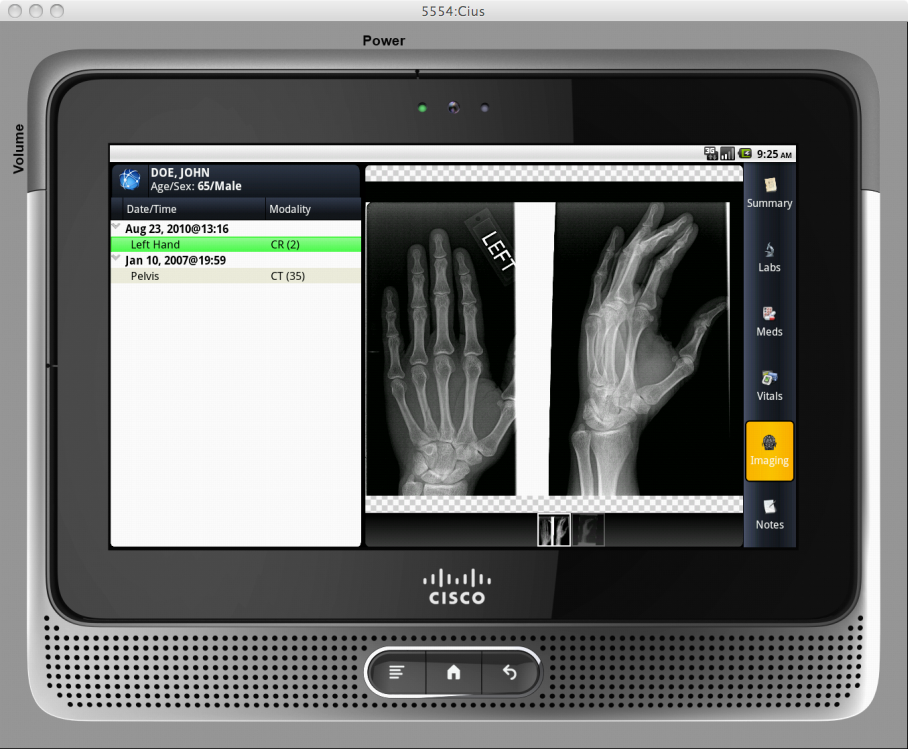
\includegraphics[width=0.5\textwidth]{pph1}
}\\
\subfloat{
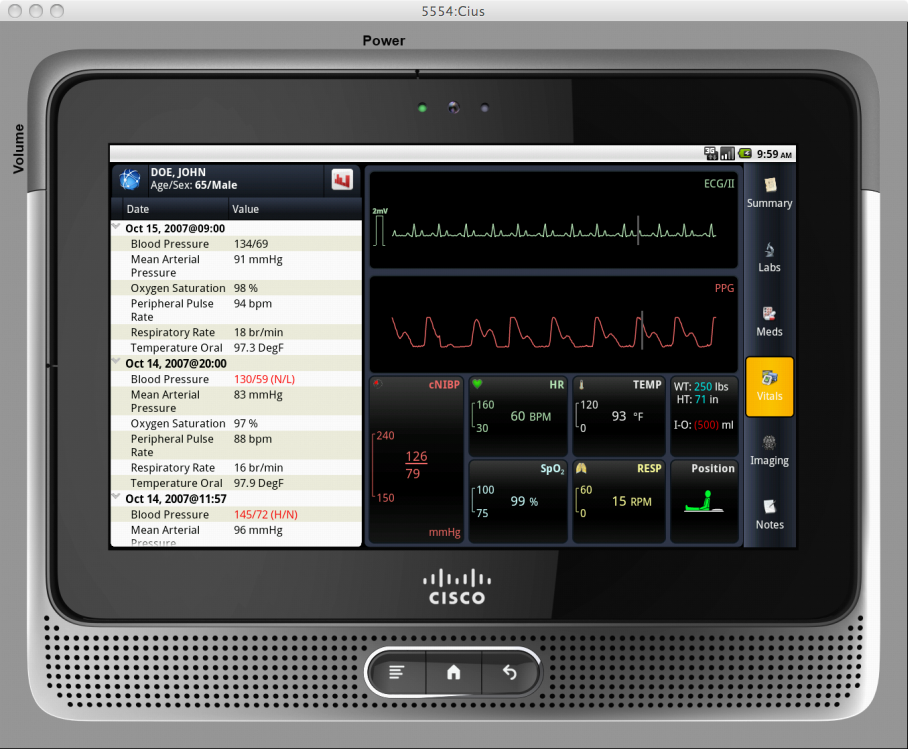
\includegraphics[width=0.5\textwidth]{pph2}
}\\
\subfloat{
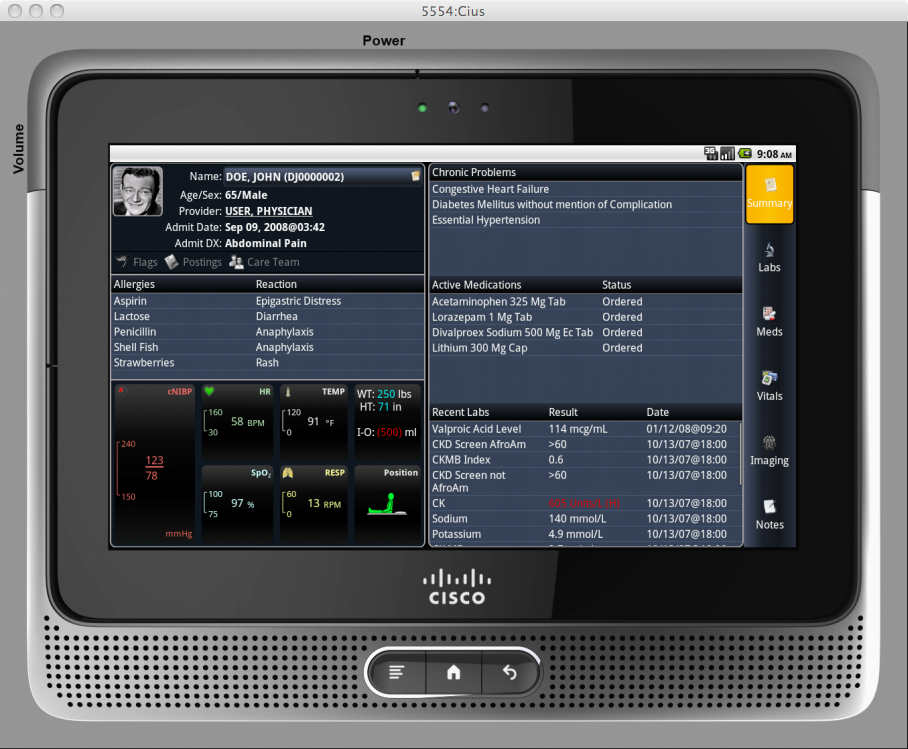
\includegraphics[width=0.5\textwidth]{pph3}
}
\caption{\gls{miaa} sur un émulateur Cisco Cius}
\label{fig:miaa}
\end{figure}

\gls{miaa} (figure \ref{fig:miaa}) est une application mobile issu d'un
projet R\&D chez \en{Palomar Pomerado Health}, l'institution public la
plus large dans l'état de Californie (USA). Elle permet aux médecins
d'accéder rapidement au dossier médical complet du patient depuis une
variété de source différentes qui s'affranchie des frontières des
organisations\cite{pph:eweek}. Elle vise les terminaux équipés avec le
système d'exploitation \android{} comme les smartphones et les
tablettes. \en{Palomar Pomerado Health} a choisi de déployer cette
application dans le \en{Palomar Medical Center} à \en{Escondido} (319
lits) et le \en{Pomerado Hospital} à \en{Poway} (107 lits) sur des
tablettes Cisco Cius\cite{pph:tabtimes}, ce choix s'est basé sur le
support qu'offre Cisco pour ces équipements.

Les avantages de \gls{miaa} sont:~\cite{pph:yahoo}

\begin{itemize}

\item Application mobile facile à utilisé conçu spécifiquement aux
médecins, tournant sur la plate-forme \android{}.

\item Un service \en{Cloud} qui fournit un accès permanent à
l'historique médicale des patients à partir de divers sources de
données qui s'affranchie des frontières des organisations.

\item Interopérabilité avec les pionniers des systèmes électroniques
de l'historique médical tel que Cerner - \tm{Millennnium},
\tm{NextGen}, et \en{Veterans Administration} - \tm{VistA}.

\item Intégration en temps-réel des technologies de surveillance
des signes vitaux sans fils comme l'ECG, SPO$_{2}$, rythme cardiaque,
température, respiration, et pression du sang à partir des équipements
sans-fils.

\item Affichage des informations génétiques personnelles.

\item Application dynamique qui s’ajuste automatiquement à l’hôpital, clinique, et à la maison.

\item Simple, facile à utiliser, avec une tactile de nouvelle génération.

\item Intégration d’une messagerie inter-médecins sécurisée tout en maintenant le contexte du patient.

\item Des plan futurs pour intégré NHIN \en{Connect} et les services
\en{Direct}.

\end{itemize}

\subsection{\pct{} - Cerner}

\begin{figure}[H]
\centering

\includegraphics[width=0.3\textwidth]{logo_cerner}
\end{figure}

\pct{} est une solution mobile conçu par le laboratoire Cerner qui
fait parti de l'ensemble de solutions \tm{Millennium+} et qui permet de
facilité le travail des médecins. Elle offre une expérience native
sur iPad pour gérer les visites médicales et permet aux médecins
d'effectuer tout une visite typique qui inclue:~\cite{pct:flyer}

\begin{itemize}

\item Consultation des emplois du temps et les chartes des patients.

\item Satisfaire les demandes récurrentes comme les commandes simples
et les recharges des médicaments.

\item Consultation des diagnostiques et résultats cliniques.

\item Documenter les allergies, les problèmes de santé et l'historique
du patient.

\item Crée et signé les notes de progressions.

\end{itemize}

Dès la fin du flux de travail du médecin ambulant. Cerner étend ces
mêmes fonctions et les adaptes aux établissements hospitaliers, les
urgences et les divers spécialistes.
Les avantages clés du \pct{} sont:~\cite{pct:flyer}

\begin{itemize}

\item Des réponses instantanées avec un flux de travail aisé.

\item Pas besoin de configurer l'application.

\item Adapter pour les visites médicales, aux patients et aux conditions
de la consultation.

\item Transmission sécurisée des données.

\item Des capacités de reconnaissance vocale.

\end{itemize}

\section{Le système d'exploitation \android{}}

\begin{figure}[H]
\begin{center}

\includegraphics[width=0.2\textwidth]{Android_robot.pdf}\\

\includegraphics[width=0.2\textwidth]{Android.pdf}
\end{center}
\caption{Logo et sigle d'\android{}}
\end{figure}

\android{} est un système d'exploitation basé sur Linux conçu pour les
équipements mobile avec d'un écran tactile comme les \en{smartphones} et
les tablettes. Développé à l'origine par \en{\android{}, Inc.} que
\en{Google} a supporté financièrement et plus-tard acquis en 2005.
\android{} a été dévoilé en 2007 parallèlement à la fondation de
l'\en{Open Handset Alliance}: un consortium composé de sociétés dévoué a
l'avancement des standards ouverts pour les équipements mobiles. Le
premier téléphone  \android{} est sorti en Octobre 2008.

La dernière version stable d'\android{} en date (Mai 2013) est 4.2.2
\en{Jelly Bean} sortie le 11 Février 2013.

\android{} est basé sur le Kernel Linux et utilise pleinement ses capacités de supports matériels exhaustifs. Mais la comparaison avec les distributions Linux, embarqué ou même destiné aux bureaux, s'arrête à ce niveau.~\cite{lft:growth_android}

\begin{figure}
\centering
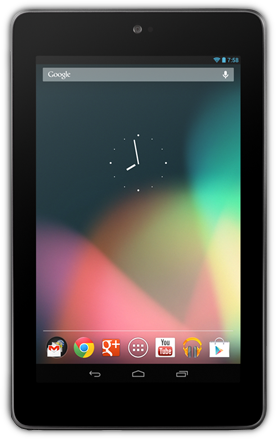
\includegraphics[width=0.4\textwidth]{nexus7}
\caption{\en{Google} Nexus 7, un terminal \android}
\end{figure}

\subsection{Parts du marché}

L’adoption du système d'exploitation \android{} suit une courbe
exponentielle depuis quelque temps et la tendance n'est pas prête de
s’inverser, selon le dernier rapport du cabinet d'analyse \en{Strategy
Analytics}, \android{} a réussi à capturer environ 68.4\% du marché
global \cite{venturebeat.com}.

\begin{table}[H]
\centering
\begin{tabular}{|m{0.2\textwidth}|m{0.13\textwidth}|m{0.13\textwidth}|m{0.13\textwidth}|m{0.13\textwidth}|m{0.13\textwidth}|}
\hline
\textsf{Système d'exploitation} &
\textsf{Volume de production 3Q2012\footnotemark[1]\footnotemark[3]} &
\textsf{Parts du Marché 3Q2012\footnotemark[1]} &
\textsf{Volume de production 3Q2011\footnotemark[2]\footnotemark[3]} &
\textsf{Parts du Marché 3Q2011\footnotemark[2]} & \textsf{Différence} \\ 
\hline
\android{} & 136.0 & 75.0\% & 71.0 & 57.5\% & 91.5\% \\
\hline
iOS & 26.9 & 14.9\% & 17.1 & 13.8\% & 57.3\% \\
\hline
BlackBerry & 7.7 & 4.3\% & 11.8 & 9.5\% & -34.7\% \\
\hline
Symbian & 4.1 & 2.3\% & 18.1 & 14.6\%  & -77.3\% \\
\hline
Windows Phone 7/ Windows Mobile & 3.6 & 2.0\% & 1.5 & 1.2\% & 140.0\% \\
\hline
Linux & 2.8 & 1.5\% & 4.1 & 3.3\% & -31.7\% \\
\hline
Autres & 0.0 & 0.0\% & 0.1 & 0.1\% & -100.0\% \\
\hline
\hline
Totales & 181.1 & 100.0\% & 123.7 & 100.0\% & 46.4\% \\ \hline
\end{tabular}

\caption{Les six major systèmes d'exploitation mobile en termes de Volume
et de parts de marché en 3\ieme trimestre 2012~\cite{idc}}

\label{tab:marketshareall}
\end{table}

\footnotetext[1]{3\ieme trimestre 2012}
\footnotetext[2]{3\ieme trimestre 2011}
\footnotetext[3]{En million d'unité}

\begin{table}[H]
\centering
\begin{tabular}{|m{0.3\textwidth}|m{0.1\textwidth}|m{0.1\textwidth}|m{0.1\textwidth}|m{0.1\textwidth}|m{0.1\textwidth}|}
\hline
& \textsf{2008} & \textsf{2009} & \textsf{2010} & \textsf{2011} &
\textsf{2012}\footnotemark[4]\\
\hline
\textsf{Unités \android{} produites} & 0.7 & 7.0 & 71.1 & 243.4 & 333.6\\
\hline
\textsf{Parts de marché \android{}} & 0.5\% & 4.0\% & 23.3\% & 49.2\%
& 68.2\%\\
\hline
\end{tabular}
\caption{Production et parts de marché entre 2008 et 2012~\cite{idc}}
\label{tab:marketshare}
\end{table}

\footnotetext[4]{Estimation}

\subsection{Versions \android{} en circulation}

Le tableau \ref{tab:androidversion} représente les différentes versions
d'\android{} et leurs taux d'utilisation respectifs. On remarque que
la plupart des terminaux mobiles \android{} sont sous la version 2.3
\en{Gingerbread} sortie le 6 Décembre 2010, Ceci est du aux fait que
plusieurs téléphones bas de gamme sont équipés de cette version et sont encore en production.

\begin{table}[H]
\centering
\begin{tabular}{|c|l|c|c|}
\hline
\textsf{Version} & \textsf{Codename} & \textsf{API} &
\textsf{Distribution}\\
\hline
1.6 & Donut & 4 & 0.2\%\\
\hline
2.1 & Eclair & 7 & 2.2\%\\
\hline
2.2 & Froyo & 8 & 8.1\%\\
\hline
2.3 - 2.3.2 & Gingerbread & 9 & 0.2\% \\
\cline{1-1}\cline{3-4}
2.3.3 - 2.3.7 & & 10 & 45.4\%\\
\hline
3.1 & Honeycomb & 12 & 0.3\%\\
\cline{1-1}\cline{3-4}
3.2 & & 13 & 1.0\%\\
\hline
4.0.3 - 4.0.4 & Ice Cream Sandwich & 15 & 29.0\%\\
\hline
4.1 & Jelly Bean & 16 & 12.2\%\\
\cline{1-1}\cline{3-4}
4.2 & & 17 & 1.4\%\\
\hline
\end{tabular}
\caption{Distribution des versions \android{} en circulation qui ont
accédé au \en{Google Play}\protect\footnotemark[5]}
\label{tab:androidversion}
\end{table}

\footnotetext[5]{Données récoltées pendant une période de tests de 14
jours arrêtée le 4 Février 2013.}
%%%ENDsubsection

\subsection[Les raisons du succès d'\android{}]{Les raisons du succès d'\android{}\cite{lft:growth_android}}

Les raisons pour le succès \android{} peuvent être
dénombrées comme suit:

\begin{description}

\item [Un \en{Framework} d'Application Riche.] \android{} fourni un
excellent \gls{sdk} avec des \gls{api} stable à long-terme, ce qui
assure aux partenaires tiers un écosystème standardisé. Alors que le
système en lui même est en constante évolution, la stabilité des
\gls{api} pour la plupart est préservée, ce qui permet d'investir dans
le long-terme. Concevoir et construire des applications pour les
distribuer sur différentes plate-formes permet des réductions drastiques en
termes des coûts et effort pour les entreprises.

\item [Un \gls{ttm} Agressif.] Concevoir des appareils avec \android{}
peut réduire le \gls{ttm} d'une manière significative. Il suffit de se
procurer les sources, les adapter pour le matériel en question et vendre. Et dans le cas ou les schémas et usages de référence sont
appliqués, la sorti d'un nouveau produit est possible au cours de quelque
mois. Seulement voilà, ce n'est pas aussi facile et une certaine expertise
et connaissances dans ce domaine sont requises. Et même si sortir un
système basé sur \android{} peut être plus rapide comparé à d'autres
solutions, le suivi des évolutions du système ainsi que maintenir le
code à long terme est une autre histoire.

\item [Concentrer sur \og Ce qui compte réellement \fg.] En fournissant
un \en{Framework} pratique, \android{} permet aux développeurs de se
concentrer sur les aspects à valeur commerciale. L'assemblage d'un
appareil est une activité qui consomme énormément de temps et de
ressources et n'a pas à réinventer un - encore - autre système d'exploitation permettant d'éviter un autre gaspillage de temps.

\item [Open Source.] Bien qu'il ne soit pas développé d'une manière
communautaire, \android{} reste 100\% modifiable et diffuse un sentiment
de sécurité parmi les entreprises contre les menaces légales.

\end{description}

\subsection[La pile logicielle d'\android{}]{La pile logicielle d'\android{}\cite{pa4ad:chptr1}}

D'une manière simple. La pile logicielle d'\android{} est un Kernel Linux et une collection de bibliothèques C/C++ exposé à travers un framework d'application qui fournit des services pour l'environnement d'exécution et les applications. On peut énumérer les éléments composant la pile logicielle comme suit:

\begin{description}

\item [Kernel Linux:]
Services de base qui inclue les pilotes matériels, gestion des processus et de la mémoire, sécurité, réseaux et gestion d'autonomie. Fourni aussi une couche d'abstraction entre le matériel et le reste de la pile.

\item [Bibliothèque:]
Se situ au dessus du Kernel, \android{} inclue divers bibliothèques C/C++ de base comme \dev{libc} et \dev{SSL} ainsi que:

\begin{itemize}

\item Une bibliothèque multimédia pour la lecture des fichiers audio et vidéo.

\item Un \en{Surface manager} pour la gestion de l'affichage.

\item Des bibliothèques graphiques qui incluent le \dev{SGL} et \dev{OpenGL} pour les graphiques 2D et 3D.

\item Un support natif de base de données à travers la base de données \dev{SQLite}.

\item \dev{SSL} et \dev{WebKit} pour le navigateur web intégrer et la sécurité internet.

\end{itemize}

\item [Environnement d'Execution (runtime) \android{}:]

L'environnement d’exécution et le facteur qui sépare un terminal \android{}
d'une implémentation Linux mobile. En cohérence avec les bibliothèques de base
et la machine virtuelle \dev{Dalvik}, l'environnement d’exécution \android{} est
le moteur qui fait fonctionner les applications et, avec les bibliothèques,
forme les bases du framework application.

\begin{description}

\item [Bibliothèque de Base:]

Même si la plus part des applications \android{} sont écrits avec du langage
\dev{Java}, \dev{Dalvik} n'est pas une machine virtuelle java. Les bibliothèques
\android{} de base fournit la plus part des fonctionnalités qu'on retrouve
dans les bibliothèques de base \dev{Java}, en plus de quelque bibliothèques
spécifiques à \android{}.

\item [La Machine Virtuelle dev{Dalvik}:]

\dev{Dalvik} est une machine virtuelle qui a était optimisé pour
s'assurer que chaque terminal peut faire fonctionner plusieurs instance
d'une manière efficace. Il s’appuie sur le Kernel Linux pour le
threading et la gestion bas niveaux de la mémoire.

\end{description}

\item [Le \en{Framework} Application:]

Le \en{Framework} application fournit les classes utilisés pour crée les application \android{}. Il fournit une abstraction générique pour l’accès matériel et gère l'\gls{ui} et les ressources de l'application.

\item [Couche Application:]

Toutes les applications, quelle soit native ou produite par un tiers, est
construites sur la couche applications via les même \gls{api}. La couche
application opère à l'intérieur de l'environnement d’exécution \android{},
utilisant les classes et les services mise à disposition par le \en{framework}
application.

\end{description}

\subsection[Architecture des applications \android{}]{Architecture des applications \android{}\cite{pa4ad:chptr1}}

L'architecture d'\android{} encourage la réutilisation des composants,
ce qui nous permet de publier et de partager des \en{Activities},
services, et données avec d'autres applications. Avec une gestion
d'accès gérée par les restrictions de sécurité que nous définissons.

Le même mécanisme qui nous permet de produire un gestionnaire de contact alternatif ou un compositeur de numéros nous permet aussi d'exposer les composants de notre application pour permettre à d'autres développeurs de les réutiliser en créant des nouveaux \gls{ui} ou d’étendre des fonctionnalités.

Les services application suivants représente les bases architecturales de toute application \android{}, fournissant le \en{Framework} qu'on va utiliser pour notre application.

\begin{description}

\item [L'\dev{Activity Manager} et le \dev{Fragment Manager}:]
Contrôle le cycle de vie de nos \en{Activities} et nos \en{Fragments} respectivement, y inclue la gestion de la pile des \en{Activities}.

\item[\dev{Views}]
Utilisé pour construire l'\gls{ui} de notre \dev{Activities} et \dev{Fragments}.

\item[\dev{Notification Manager}:]
Fournit un mécanisme consistant et non-intrusif de signalisation pour l'utilisateur.

\item[\dev{Content Providers}:]
Permet à notre application le partage des données.

\item[\dev{Resource Manager}:]
Offre un moyen d'externaliser les ressources (comme par exemple les chaînes de caractères et les images.)

\item[\dev{Intents}:]
Présente un mécanisme pour transférer les données entre les applications et leurs composants.

\end{description}

Une des fonctionalités les plus intéressantes pour l'aboutissement de notre projet offerte par \android{} sont ses capacités de localisation, étudiées dans la partie suivante.

\subsection{Location Based Services}

\subsubsection{Concept}

Pour positionner un terminal, on spécifie ses coordonnées géographiques
en utilisant le géo-codage.

\paragraph[Géo-codage]{Géo-codage\cite{wiki:geocoding}}

Le géo-codage est le processus de retrouver les coordonnées
géographiques associées (exprimées souvent en terme de \textit{latitude}
et \textit{longitude}) d'après d'autre données géographiques comme
l'adresse de la rue, code postal. Ces coordonnées géographiques peuvent
être insérées dans un système d'informations géographiques ou intégré dans
des médias comme les photos numériques par le biais de géo-marquage.
Cette opération est communément appelé le \en{Forward Geocoding}.

Le \en{Reverse Geocoding} est la procédure inverse: retrouvé les lieux textuel comme l'adresse de la rue d'après les coordonnés géographiques. Car même si l'usage des paramètres comme la longitude et la l'attitude fourni un moyen pratique pour localisé l'individu d'une maniéré relativement précise. Les utilisateurs penche à pensés en terme de rues et adresses.

A fin de déterminer la position du terminal, plusieurs technologie de localisation sont à notre disposition.

\paragraph[Localisation par GSM]{Localisation par GSM}

On peut retrouver la position du terminal mobile par le biais de sa
cellule \gls{gsm}. Cette technique fait intervenir divers moyens de
triangulation des signaux parvenant depuis les cellules qui desservent
un téléphone mobile. La position géographique du terminal est déterminée
par une multitude de méthodes comme la \gls{tdoa} ou l'\gls{e-otd}.

\paragraph[Localisation parGPS]{Localisation parGPS\cite{enig:gps}}

\gls{gps} est un système de navigation par satellites qui fourni la
localisation et le temps dans toute condition météorologique et partout
sur terre s'il existe un accès non bloquant à 4 ou plus satellites
\gls{gps}. Ce Système fourni des services essentiels dans le domaine
militaire, civil et commercial partout dans le monde. Il est maintenu
par les États Unis d'Amérique et accessible à quiconque possédant un
récepteur \gls{gps}.

\subsubsection[La localisation dans \android{}]{La localisation dans \android{}\cite{pa4ad:chptr13}}\label{sss:android_localisation}

L'accès aux \gls{lbs} se fait essentiellement via deux objets:
\begin{description}
\item [\dev{Location Manager}]\footnote{android.location.LocationManager} Permet d'exploiter les services basés sur la localisation.
\item [\dev{Location Providers}]\footnote{android.location.LocationProvider} Chaque \en{Providers} représente une technologie de localisation utilisé afin de déterminer la localisation actuel du terminale.

\end{description}
On utilise ces deux Classes pour les fins suivantes:
\begin{itemize}
\item Obtenir la position actuelle.
\item Suivre les mouvements.
\item Alerte de proximité dans le cas ou l'on approche ou s’éloigne d'une zone spécifique.
\item Retrouver les fournisseurs de localisation disponible.
\item Observer le status du récepteur \gls{gps}.
\end{itemize}

Généralement deux techniques de détection de localisation sont disponibles dans le terminal: détection par le réseau \en{Network Provider} et la détection par \gls{gps} (\en{GPS Provider}). Le choix de la technologie à utiliser est soit explicite ou automatique suivant des critères prédéfinis par le développeur de l'application. Avant de pouvoir exploiter un service de localisation, un niveau de précision doit figurer dans le manifeste de l'application via les \dev{uses-permission} \en{tags}.

\paragraph{Niveau de permission \textbf{COARSE} } % (fold)
\label{par:coarse}

\begin{lstlisting}[language=xml, caption=Permission pour la localisation par le réseau.]
<uses-permission android:name="android.permission.ACCESS_COARSE_LOCATION"/>
\end{lstlisting}
% paragraph par:coarse (end)

\paragraph{niveau de permission \textbf{FINE} } % (fold)
\label{par:fine}

\begin{lstlisting}[language=xml, caption=Permission pour la localisation par GPS.]
<uses-permission android:name="android.permission.ACCESS_FINE_LOCATION"/>
\end{lstlisting}

A noter qu'une application ayant la permission \dev{FINE} possède implicitement la permission \dev{COARSE}.

Avoir la localisation dans la plat-forme \android{} se fait par le biais de
\en{callback}, on indique au \dev{LocationManager} qu'on veut recevoir des mise
à jour de la localisation par la fonction \dev{requestLocationUpdates()} en lui
passant une implémentation de
\dev{LocationListener}\footnote{android.location.LocationListener}. Cette
interface contient plusieurs fonctions de \en{callback} que le
\dev{LocationManager} appelle quand la localisation de l'utilisateur change ou
l'état du service change\cite{guide:location_strategies}.


\section{Conclusion}

Dans ce chapitre, on s'est permis d'inspecter les solutions similaires à
la notre dans le but de s'éclaircir les idées sur les problèmes qu'on
pourrait rencontrer et pour mieux cerner les difficultés que nous allons
rencontré. Vient en suite la présentation de la plate-forme ciblée en
plus d'une application type, des connaissances critiques pour le chapitre
suivant qui porte sur le travail effectué.

%!TEX root = report.tex

\chapter{Analyse des besoins}


Dans ce chapitre on présente les environnements logiciels et matériels dans lesquelles s'est dérouler le développement de l'application ainsi qu'une étude des besoins effectué pour cerner nos objectifs.

\section{Environnement de développement}%TODO

Plusieurs outils ont été mises à contribution pour développer l'application, tant sur le plan logiciel que matériel.

\subsection{Environnement Logiciel}
Voici une liste des outils logiciels utilisés pendant le développement de l'application.

\begin{description}

\item [Ubuntu 12.04] Système d'exploitation.\footnotemark[1]

\item [OpenJDK 6] \gls{jdk} version 6.\footnotemark[2]

\item [Eclipse Juno] Environnement de Développement Intégré dans sa version \en{Service Release 2}.\footnotemark[3]

\item [\gls{adt} (plugin Eclipce)] Intégration des outils de développement fournit dans l'\gls{sdk} \android{}.\footnotemark[4]

\item [ObjectAid (plugin Eclipce)] Génération des diagrammes de classes.\footnotemark[5]

\item [PlantUML (plugin Eclipce)] Génération des diagrammes de séquences.\footnotemark[6]

\item [Git] Gestionnaire des versions\footnotemark[7].

\item [EGit (plugin Eclipse)] Intégration du gestionnaire de version.\footnotemark[8]

\item [Evolus Pencil] Génération de prototypes et des sketchs\footnotemark[9]
\end{description}

\footnotetext[1]{http://www.ubuntu.com}
\footnotetext[2]{http://openjdk.java.net}
\footnotetext[3]{http://www.eclipse.org}
\footnotetext[4]{https://developer.android.com/tools/sdk/eclipse-adt.html}
\footnotetext[5]{http://www.objectaid.com/}
\footnotetext[6]{http://plantuml.sourceforge.net/}
\footnotetext[7]{ttp://git-csm.com}
\footnotetext[8]{http://www.eclipse.org/egit/}
\footnotetext[9]{http://pencil.evolus.vn/}

\subsection{Environnement Matériel}

Le développement de l'application est fait avec une tablette Asus Nexus 7 (mise à jour à \android{} 4.2.2 \en{Jelly Bean}).


\section{Étude des Besoins}

\subsection{Besoins fonctionnels}

\begin{figure}[H]
\center
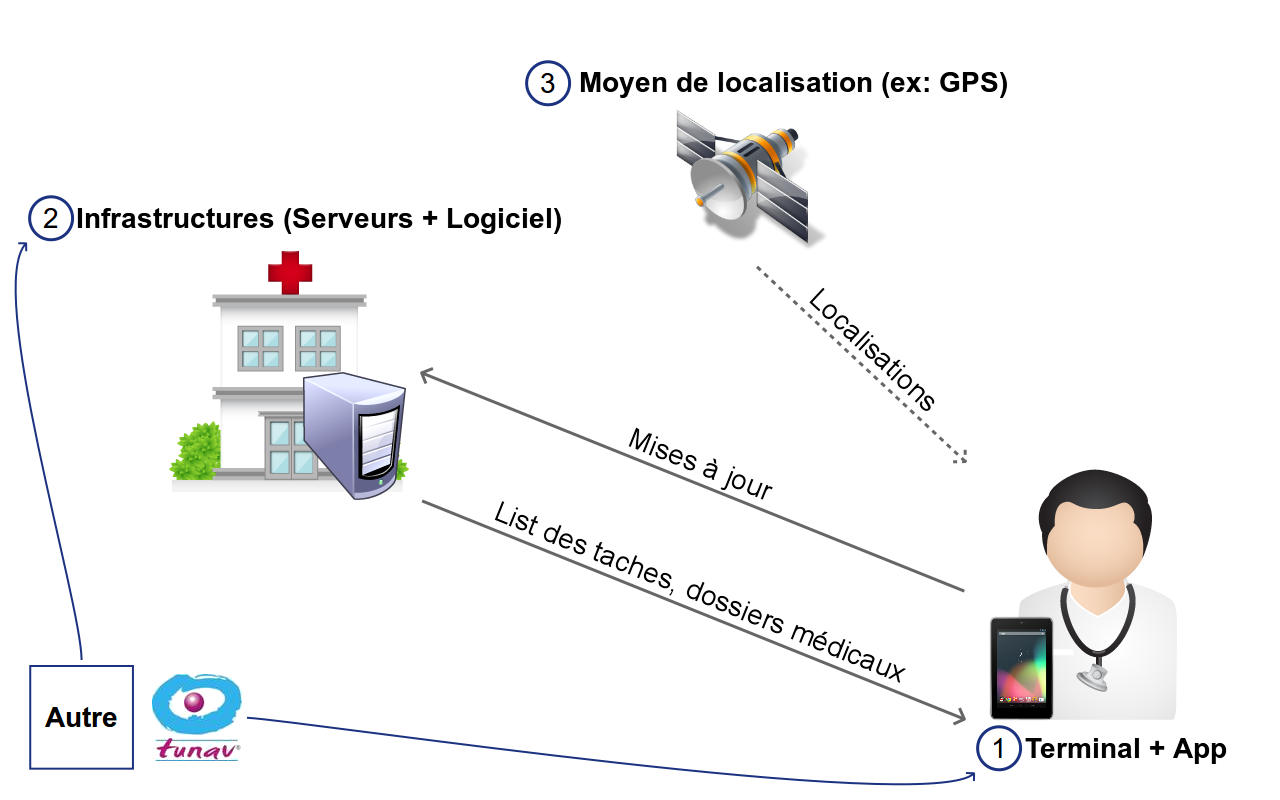
\includegraphics[width=0.8\textwidth]{scenario-other}
\caption{Illustration des besoins fonctionnels.}
\end{figure}

\begin{itemize}

\item Le médecin doit être capable à partir de son terminal d’avoir des
informations sur les patients qui lui sont assignés en fonction de leur position
géographique.

\item L'application doit être capable de détecter la proximité d'un
patient en fonction de la position actuelle du terminal.

\item Le médecin peut télé-consulter le dossier médical du patient.

\end{itemize}

\subsection{Besoins non fonctionnels}

\begin{itemize}

\item Une bonne ergonomie qui vise à faciliter l'obtention de
l'information, avec un minimum d'effort pour l'utilisateur cible et
avec le moindre risque d'erreur. Les choix graphiques et conceptuels
sont des considérations à tenir en compte.

\end{itemize}

\subsection{Besoins techniques}

\begin{figure}[H]
\center
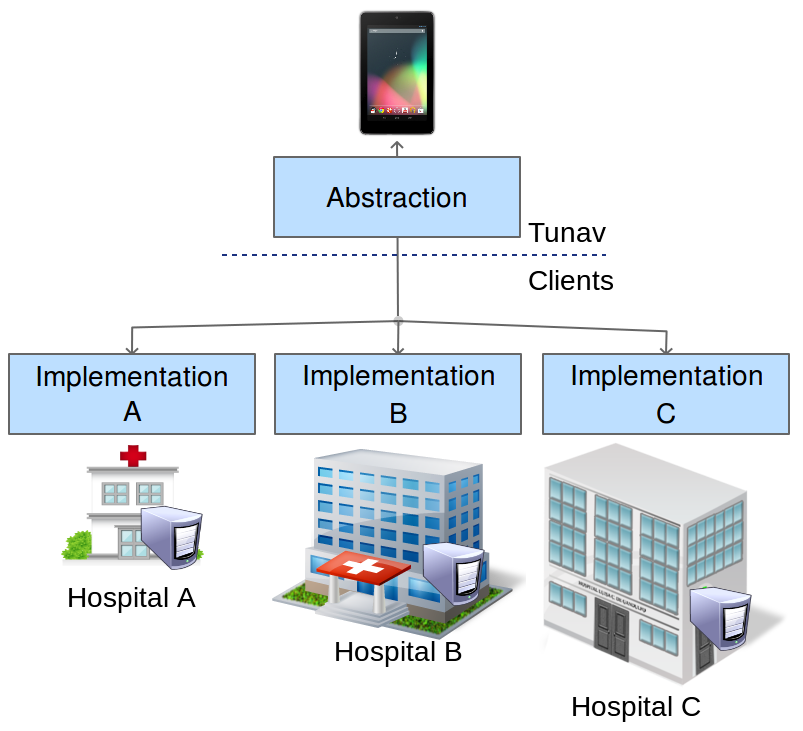
\includegraphics[width=0.8\textwidth]{architecture-interfaces}
\caption{Illustration des besoins techniques.}
\end{figure}

\begin{itemize}

\item L’application mobile vise à utiliser les systèmes déjà en place des
établissements clients pour réduire les coûts. Vu l’absence d'un protocole
standards et les différentes implémentations possibles des différents clients,
l'implémentation d'une couche d’accès abstraite est requise pour pouvoir
déployer l’application avec le minimum de modification.

\end{itemize}

\subsection{Identification des acteurs}

Notre système interagit essentiellement avec trois acteurs différents:

\begin{description}

\item[Le médecin] C'est l'acteur principal de notre système.

\item[Le service web] Source des données à acheminer vers le médecin.

\item[Système d'exploitation] Communique à notre système les
informations recueillies des divers composants qui nous intéressent
(localisation GPS/Network, état de la connectivité, état de la
batterie).

\end{description}

\subsection{Cas d'utilisations}

On peut présenter les interactions fonctionnelles entre les acteurs gouverné par leurs besoins avec un diagramme des cas d'utilisations (figure \ref{fig:uml_usecase}).

\begin{figure}
\center
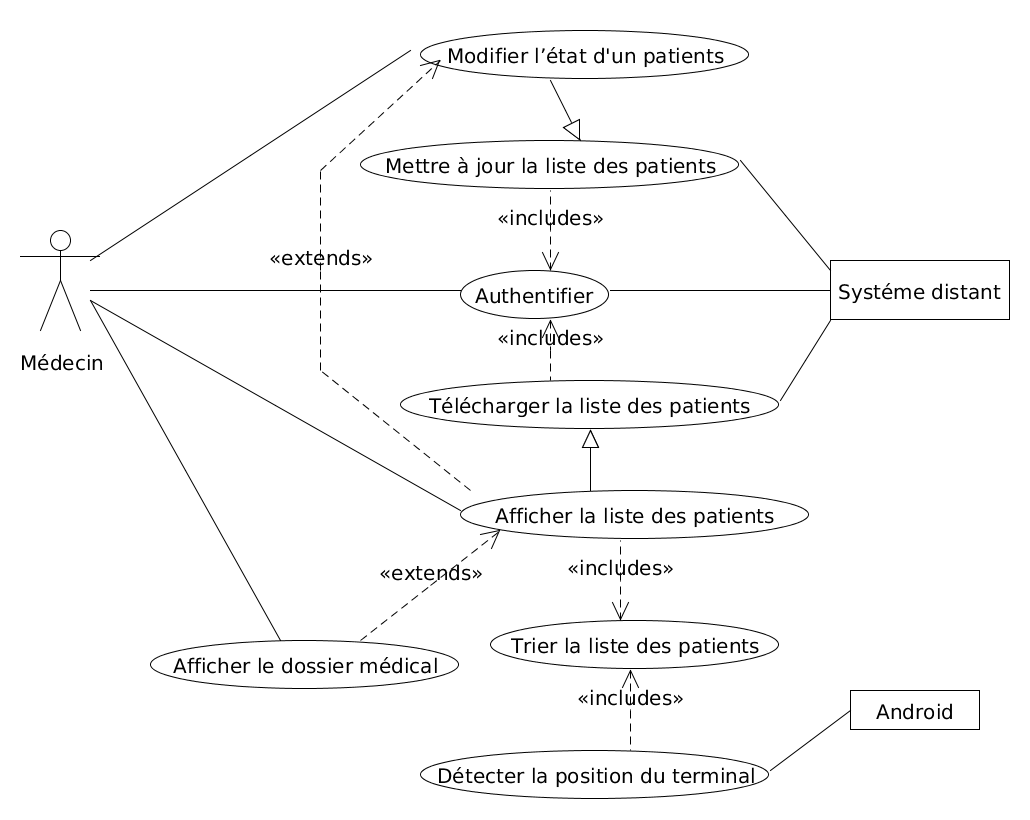
\includegraphics[width=0.8\textwidth]{diagrams/usecases}
\caption{Diagramme des cas d'utilisation \gls{uml} globale.}
\label{fig:uml_usecase}
\end{figure}
%!TEX root = report.tex

\chapter{Études Structurels}

\section{Introduction du chapitre}

\section[Couche d'Accès aux Données]{Couche D'Accés aux Données}

Un des objectifs principales de ce projet étant de fournir une solution
d’accès aux données flexibles à fin de couvrir les besoins de chaque
client de manière individuelle. On a opté donc pour un modèle basé sur
l’implémentation de deux interfaces (figure \ref{fig:cls_dal}):

\begin{itemize}

\item Interface d'authentification.

\item Interface d’accès à la liste des patients.

\end{itemize}

\begin{figure}
\center
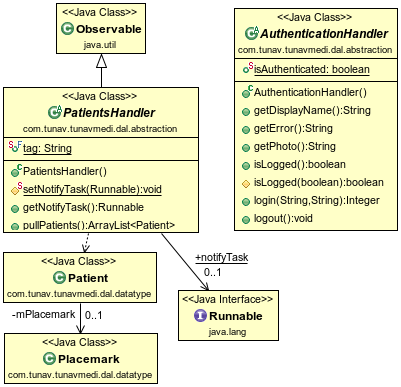
\includegraphics[totalheight=0.5\textheight]{diagrams/cls_dal}
\caption{Diagramme de classes \gls{uml} des interfaces de la couche d’accès.}
\label{fig:cls_dal}
\end{figure}

L'idée est simple: pour chaque client, une implémentation spécifique à son infrastructure sera développée soit par son propre effectif, soit par une des équipes de \textsc{Tunav}, ou dans le cas idéal par une alliance formé par des agents des deux camps qui garantie une collaboration plus poussée pour des résultats meilleurs.
Ces ensembles d'interfaces nous permettent de construire notre application.

\subsection{Interface d'authentification}

\dev{AuthenticationHandler}\footnotetext{com.tunav.tunavmedi.dal.abstraction.AuthenticationHandler} (figure
\ref{fig:cls_dal}) est une classe abstraite comportant les méthodes
requise par notre application pour effectué les actions
d'authentification, de dé-authentification, de vérification
d'authenticité ainsi l'obtention des informations associées à l'utilisateur
authentifier.

Malgré la variété des techniques d'authentification utilisée dans le domaine
informatique, l'étape d'acquisition des identificateurs de l'utilisateur
représente un point de départ commun. On utilise ce caractère dans l'interface
d'authentification en demandant à nos clients d'implémenter la méthode
\dev{login()} qui prend en argument l'identifiant et le mots de passe fourni par
le médecin, dans le cas d'une éventuelle erreur d'authentification,
l’implémentation met a notre disposition un message d'erreur accessible par la
méthode \dev{getError()}. Pour effectuer l’opération inverse le client
implémente la méthode \dev{logout()} supposée annoncer au service distant la dé-
authentification de l'utilisateur du terminal. Pour vérifier le l'état actuel de
la relation du terminal avec la base distante, on utilise le booléen retourné
par \dev{getStatus()}, utile dans les cas de déconnexion temporaire ou du
redémarrage de notre application. Les méthodes \dev{getDisplayName()} et
\dev{getPhoto()} retournent respectivement le nom de l'utilisateur et sa photo.

\subsection{Interface d’accès à la liste des patients}

\dev{PatientsHandler}\footnotetext{com.tunav.tunavmedi.dal.abstraction.PatientsH
andler} (figure \ref{fig:cls_dal}) est une classe abstraite comportant les
méthodes requises par notre application pour effectuer les actions de mise à
jour de la liste des patients dans le deux sens (terminal $\rightarrow$ service
et terminal $\leftarrow$ service), elle contient aussi un objet de type
\dev{Runnable}\footnotetext{java.lang.Runnable} associé au mécanisme de notification.

\subsubsection{Mécanisme de notification}

Le patron \textbf{Observateur} (\en{observer pattern}) (fig
\ref{fig:observer}) et un patron de conception couramment utilisé et qui
nous permet d'avoir une relation 1$\rightarrow$N entre divers objets. Le
patron observateur assume que l'objet qui contient les données est
séparé des l’objet qui les affiche et ces dites objets observe le
changement de ces données~\cite{jdp_observer}. Quand on implémente le
patron observateur, on réfère communément à l'objet contenant les
données par "Sujet"; et chacun des consommateurs des données par
"Observateur", Et chaque Observateur implémente une interface préconçu
que le Sujet invoque quant les données changent~\cite{jdp_observer}.

\begin{figure}[H]
\center
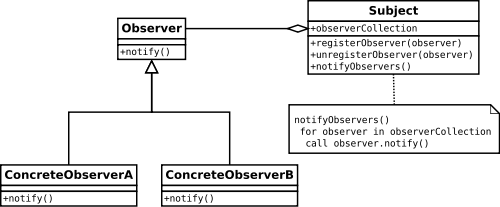
\includegraphics[width=0.8\textwidth]{Observer}
\caption{Diagramme \gls{uml} du patron de conception Observateur~\cite{wikipedia:observer}}
\label{fig:observer}
\end{figure}

Dans le langage Java, ce patron est réalisé à travers la classe \dev{java.util.Observable} et l'interface \dev{Observer}\footnotetext{Java.util.Observer}. Le Sujet hérite de la classe \dev{Observable} et les changements sont signalés par les méthodes \dev{setChanged()} et \dev{notifyObservers()} ou \dev{notifyObservers(Object message)}.

\subsubsection{Les objets de données}

\begin{figure}
\center
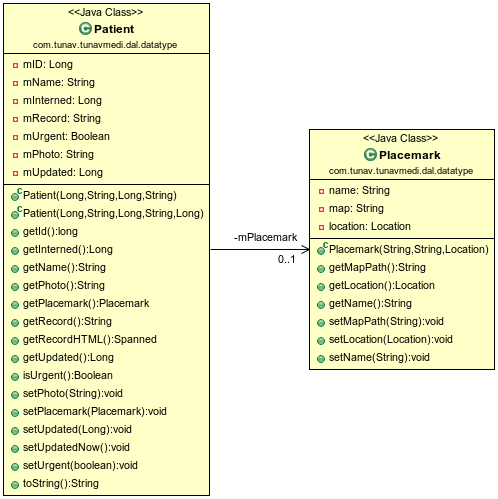
\includegraphics[width=0.8\textwidth]{diagrams/cls_dal_patient}
\caption{Diagramme de la classe \gls{uml} \dev{Patient} }
\label{fig:cls_dal_patient}
\end{figure}

La communication des données avec le service distant se fait à travers l'objet \dev{Patient}\footnotetext{com.tunav.tunavmedi.dal.datatype.Patient} (figure \ref{fig:cls_dal_patient}. Cet objet contient toutes les informations requises pour la synchronisation et l'affichage et la gestion des patients, en particulier le dossier médical et la position actuelle du patient.

\paragraph{Synchronisation:}

Étant sujet aux modifications de la part de l'application et du serveur distant, Un problème se pose pour connaître la version la plus à jour. Pour cela chaque modification apportée est suivi par une mise à jour de variable \dev{mUpdated} par le temps à cette instance précise (cette opération est interne à l'objet). En cas ou deux versions différentes de l'objet \dev{Patient} avec le même \dev{mID} et \dev{mUpdated}, le service est supposé favoriser sa version.

\paragraph{Dossier médical:}

Le dossier médical est fourni sous le format \en{HTML}. Cette représentation est idéale car elle nous permet de faire abstraction sur le format du dossier tel que sauvegardé par l'établissement client, la couche d’accès assurant éventuellement la conversion.


\paragraph{Position:}

La position actuelle du patient est représentée par un objet \dev{Placemark}\footnote{com.tunav.tunavmedi.dal.datatype.Placemark} inspiré par la notation XML \gls{kml}. Les coordonnées sont représentées par un objet de type \dev{Location}\footnote{android.location.Location}.

\subsection{Implémentation de tests}\label{subsection:dal_impl}

Le package \dev{com.tunav.tunavmedi.dal.sqlite} contiens une
implémentation de la couche d’accès abstraite (figure
\ref{fig:dal_sqlite}) réalisée dans le cadre de ce projet pour
pouvoir tester la solution. Cette implémentation est de caractère local
à l'application à travers les \gls{api} de la base de données
\dev{SQLite} qui fait partie de l'\gls{sdk} \android{}. En fait une
implémentation locale nous affranchie des problèmes qui peuvent se
produire et dont la corrélation avec l'application est faible. Cette même
idée a influencé la mise en place même de cette implémentation qui à su
rester la plus simple possible en restant très proches des objets de
base de notre application.

\begin{figure}
\center
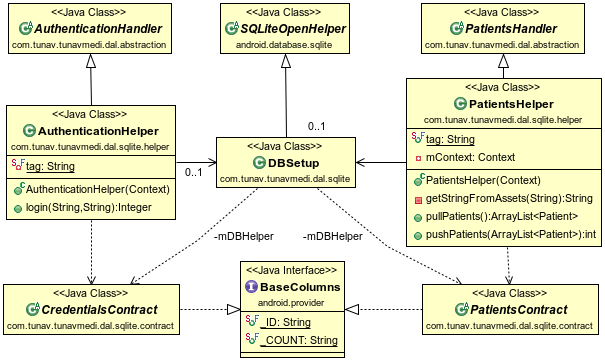
\includegraphics[angle=-90, width=0.8\textwidth]{diagrams/cls_dal_sqlite}
\caption{Diagramme de classe de l'implémentation de la couche d'accès de tests  à base de SQLite.}
\label{fig:dal_sqlite}
\end{figure}

Cette implémentation peut être subdivisée en trois éléments: Les \dev{Contrats}, les \dev{Helpers}, et la classe \dev{DBSetup}.

\paragraph{Les Contrats:}

Représente les contrats relatifs aux tables dans notre implémentation de
tests. Chaque contrat implémente l'interface
\dev{BaseColumns}\footnote{android.provider.BaseColumns} et contient - entre autre - les
commandes SQL de création et de suppression de la dite table, des
éventuels index, et les commande d'insertion des données de test.

\paragraph{Les \en{Helpers}:} 

Ce sont les implémentations des classes abstraites qui définissent la
couche d’accès et présentent les procédures d'extraction des données pré-
insérées dans nos tables fictives en faisant appel à la classe
\dev{DBSetup} .

\paragraph[La classe \dev{DBSetup}:]{La classe \dev{DBSetup}:} 

Elle hérite de la classe \dev{SQLiteOpenHelper} et est destinée à
contrôler la création et l’accès à notre base de données de tests.

\section{Structure de l'Application}

L'application est subdivisée en deux parties majeures représentés par deux classes de type \dev{Activity}\footnotetext{android.app.Activity} :

\begin{description}

\item [LoginActivity:] C'est une entité indépendante qui implémente la logique d'authentification, 

\item [MainActivity:] C'est l'entité principale de notre solution mobile, elle relie les divers composants utilisés dans la transmission de la liste des patients, de la localisation et de la Conscience de l'état du terminal.

\end{description}

\subsection{LoginActivity}

%TODO AsyncTask

\begin{lstlisting}[language=xml, caption=Déclaration de LoginActivity dans AndroidManifest]

        <activity
            android:name="com.tunav.tunavmedi.activity.LoginActivity"
            android:label="@string/app_name"
            android:screenOrientation="portrait" >
            <intent-filter>
                <category android:name="android.intent.category.DEFAULT" />

                <action android:name="com.tunav.tunavmedi.action.LOGOUT" />
                <action android:name="com.tunav.tunavmedi.action.LOGIN" />
            </intent-filter>
        </activity>

\end{lstlisting}

\subsection{MainActivity}

\begin{lstlisting}[language=xml, caption=Déclaration dans AndroidManifest de MainActivity]

        <activity
            android:name="com.tunav.tunavmedi.activity.MainActivity"
            android:label="@string/title_activity_main"
            android:screenOrientation="portrait" >
            <intent-filter>
                <action android:name="android.intent.action.MAIN" />

                <category android:name="android.intent.category.DEFAULT" />
                <category android:name="android.intent.category.LAUNCHER" />
            </intent-filter>
        </activity>

\end{lstlisting}

L'architecture globale du \dev{MainActivity}  (figure \ref{fig:cls_global})
est calquée sur Le patron "Vue Passive" (Passive View Pattern). Le patron
\en{Passive View} (fig \ref{fig:passive_view}) est une variation des
patrons \gls{mvc} et \gls{mvp}, de ce qui ce passe dans ces patrons.

L'interface utilisateur est divisée entre une Vue qui s'occupe de
l'affichage des données et un contrôleur qui répond aux interactions de
l'utilisateur. La différence majeur avec le \en{Passive View} est que la
Vue est complètement passive et n'est pas responsable de sa mise à jour
depuis le modèle. Dans ce cas toute la logique de la Vue est dans le
contrôleur et aucune dépendance ni dans un sens au dans un autre entre
la Vue et le modèle~\cite{fowler:passive_view}.

\begin{figure}
\center
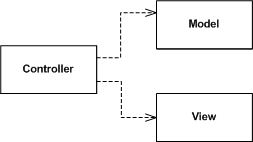
\includegraphics[width=0.6\textwidth]{passive_view}
\caption{Diagramme \gls{uml} de composants du patron \en{Passive View}~\cite{fowler:passive_view}}
\label{fig:passive_view}
\end{figure}

Ce patron est idéal dans notre cas pour deux raisons majeures:

\begin{itemize} 

\item Dans notre projet la Vue n'est pas la partie la plus importante
dans la mesure où l'objectif est d'intégrer un système développé
parallèlement, donc éventuellement avec une autre logique de
présentation. Déporter les interactions avec le modèle dans le
contrôleur permet d'intégrer d'autres implémentations d'affichage plus
facilement.

\item La nature même de cette procédure d’accès - à savoir l’aspect
abstrait, donc plus fragile - nous conduit à réduire les composants en
relations pour réduire la marge d'erreur possible et facilité les tests d’intégration.

\end{itemize}

\begin{figure}
\center
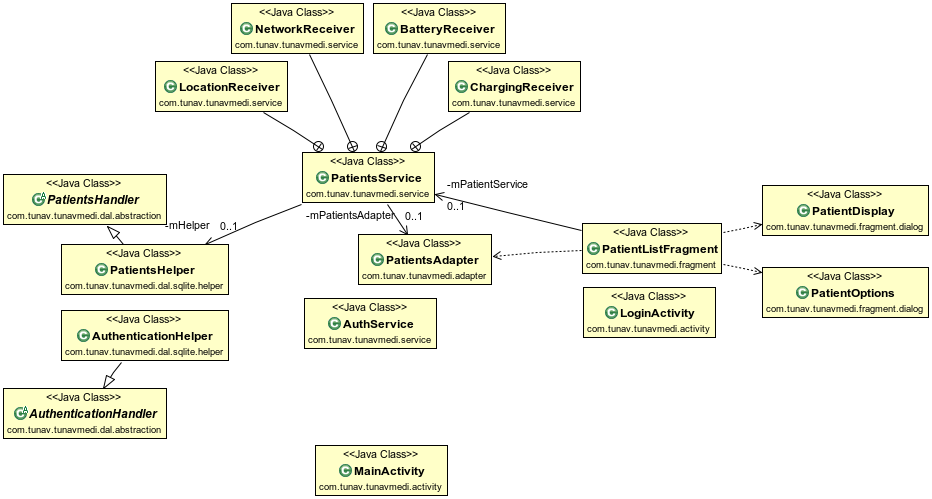
\includegraphics[angle=-90, width=0.9\textwidth]{diagrams/cls_global}
\caption{Diagramme de classes \gls{uml} de l'architecture générale de l'application.}
\label{fig:cls_global}
\end{figure}

Dans la suite de ce chapitre, on procède à l'explication détaillée du Contrôleur
et de la Vue, pour le Modèle se vous reporter au point
\ref{subsection:dal_impl}.

\subsubsection{Le Contrôleur}

\begin{figure}
\center
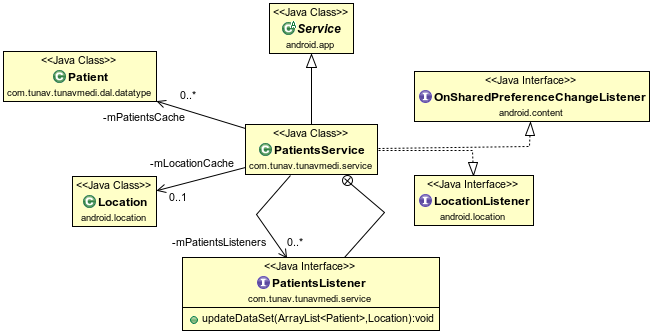
\includegraphics[width=0.8\textwidth]{diagrams/cls_ctrl}
\caption{Diagramme \gls{uml} de classe du contrôleur.}
\label{fig:cls_ctrl}
\end{figure}

\begin{lstlisting}[language=xml, caption=Déclaration dans AndroidManifest du PatientService]

        <service
            android:name="com.tunav.tunavmedi.service.PatientsService"
            android:exported="false" >
            <intent-filter>
                <category android:name="android.intent.category.DEFAULT" />
            </intent-filter>
        </service>

\end{lstlisting}

Notre contrôleur est matérialisé par l'objet
\dev{PatientService}\footnote{com.tunav.tunavmedi.service.PatientService} qui
hérite de la classe \dev{Service}\footnote{android.app.Service}. L'\gls{api}
\android{} définie un service comme étant un composant de l'application qui
représente soit la volonté de cette application de faire des longues opérations
sans interagir avec l'utilisateur ou d’offrir des fonctionnalités à
l'intention des autres applications\cite{api:service}.

\paragraph{Localisation:}
Pour la localisation, le contrôleur implémente les techniques présentées dans \ref{sss:android_localisation}
%TODO

\paragraph{Conscience de l'état du terminal}

Le tableau \ref{tab:status} représente la configuration que le contrôleur suit dans le cas d'un changement d’état du terminal. En particulier l'inutilité de chercher la position actuelle du terminal dans le cas ou celui ci est en charge, encore en cas ou le terminal annonce que la batterie est faible, on procède à un mode d’économie d’énergie pour éviter entre autres la corruption des données.

\begin{table}[H]
\centering
\begin{tabular}{|c|c|c|}
\hline
&\textsf{Mises à jour} & \textsf{Localisation}\\
\hline
\textsf{Batterie Faible} & déactivé & déactivé\\
\hline
\textsf{Batterie en Charge} & activé & déactivé\\
\hline
\textsf{Pas de connectivité} & déactivé & activé\\
\hline
\end{tabular}
\caption{Configuration du contrôleur en réponse au changement d’état du terminal}
\label{tab:status}
\end{table}

\subparagraph{Connectivité:}

Les permissions citées dans le listing \ref{lst:permission_network} sont nécessaires pour s’abonner aux événement liés à la connectivité du terminal. Le \dev{NetworkReceiver}\footnote{com.tunav.tunavmedi.broadcastreceiver.NetworkReceiver} (listing \ref{lst:receiver_network}) s'occupe de notifier les intéressés, dans notre cas le contrôleur, via des \dev{SharedPreferences}.

\begin{lstlisting}[language=xml, label=lst:permission_network, caption=Déclaration dans AndroidManifest des permissions d’accès à l’état des interfaces réseaux.]

<uses-permission android:name="android.permission.ACCESS_NETWORK_STATE" />

\end{lstlisting}

\begin{lstlisting}[language=xml, label=lst:receiver_network, caption=Déclaration dans AndroidManifest du  NetworkReceiver]

        <receiver
            android:name="com.tunav.tunavmedi.broadcastreceiver.NetworkReceiver"
            android:enabled="true" >
            <intent-filter>
                <action android:name="ConnectivityManager.CONNECTIVITY_ACTION" />
            </intent-filter>
        </receiver>

\end{lstlisting}

\subparagraph{Batterie}

Le \dev{BatteryReceiver}\footnote{com.tunav.tunavmedi.broadcastreceiver.BatteryReceiver} (listing \ref{lst:receiver_battery}) fait savoir au contrôleur via des \dev{SharedPreferences} si la batterie est faible ou pas.

\begin{lstlisting}[language=xml, label=lst:receiver_battery, caption=Déclaration dans AndroidManifest du BatteryReceiver.]

        <receiver
            android:name="com.tunav.tunavmedi.broadcastreceiver.BatteryReceiver"
            android:enabled="true" >
            <intent-filter>
                <action android:name="android.intent.action.BATTERY_LOW" />
                <action android:name="android.intent.action.BATTERY_OK" />
            </intent-filter>
        </receiver>

\end{lstlisting}

\subparagraph{Mobilité:}
Le \dev{ChargingReceiver}\footnote{com.tunav.tunavmedi.broadcastreceiver.ChargingReceiver} (listing \ref{lst:receiver_network}) est destiné à notifier le contrôleur quand le terminal est connecté ou déconnecté du  chargeur via des \dev{SharedPreferences}.

\begin{lstlisting}[language=xml, label=lst:receiver_charging, caption=Déclaration dans AndroidManifest ChargingReceivers.]

        <receiver
            android:name="com.tunav.tunavmedi.broadcastreceiver.ChargingReceiver"
            android:enabled="true" >
            <intent-filter>
                <action android:name="android.intent.action.ACTION_POWER_CONNECTED" />
                <action android:name="android.intent.action.ACTION_POWER_DISCONNECTED" />
            </intent-filter>
        </receiver>

\end{lstlisting}

\subsubsection{La Vue}

\begin{figure}
\center
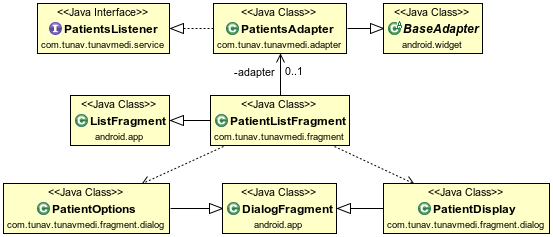
\includegraphics[width=0.8\textwidth]{diagrams/cls_view}
\end{figure}

Le système d'exploitation \android{} rend facile le développement des applications qui tournent sur des appareils qui possèdent des formes et des tailles d’écrans différentes, une des améliorations apportées dans \android{} 3.0 Honeycomb sont les \dev{Fragment} censé décomposé les fonctionnalité et les interfaces utilisateur d'une l'application \android{} en des modules réutilisables. Notre implémentation de la Vue prend avantage de cette introduction en utilisant des \dev{Fragments} et se compose essentiellement de 4 composants:

\begin{description}

\item[PatientAdapter] Représente un \dev{BaseAdapter} qui joue le rôle d'un adaptateur entre la \dev{PatientListFragment} et notre contrôleur, la communication avec celui-ci est assuré à travers l'interface \dev{PatientsListener}.

\item[PatientListFragment] Hérite de l'objet \dev{PatientListFragment} et s'occupe de l'affichage de la liste des patients.

\item[PatientDisplay] Un \dev{DialogFragment} qui s'occupe de l'affichage du dossier médical du patient

\item[PatientOptions] Un \dev{DialogFragment} qui permet au docteur de modifier la condition d'un patient.

\end{description}

\paragraph{Algorithme de Trie}

L'or de l'affichage de la liste des patients, une opération de trie est appliquée pour faciliter la tache du docteur en mettant en valeur les cas qui requièrent le plus son attention.
L’algorithme se base sur les conditions suivantes (dans l'ordre):

\begin{enumerate}

\item Le patient est un cas urgent ou non.

\item Le patient est à proximité ou non.

\item La date d'admission du patient.

\end{enumerate}

Cette opération est réalisé la méthode static \dev{java.util.Collections.sort()} en utilisant notre propre objet de type \dev{java.util.Comparator<Patient>} qui respecte les conditions citées ci-dessus.


\paragraph{Affichage du dossier médical}

Le dossier étant sous la forme d'un document HTML, pour l'afficher on utilise un \dev{WebView}\footnote{android.webkit.WebView} (listing \ref{lst:xml_patientdisplay})qui nous offre les capacités d'affichage d'un vrai navigateur web.


\begin{lstlisting}[language=xml, label=lst:xml_patientdisplay, caption=Déclaration XML du WebView utilisé par PatientDisplay]

    <WebView
        android:id="@+id/task_dialog_description"
        style="@style/ListDescription"
        android:layout_width="match_parent"
        android:layout_height="wrap_content"
        android:layout_below="@id/task_dialog_separator"
        android:textIsSelectable="true" 
        android:singleLine="false"/>

\end{lstlisting}

\section{Conclusion du Chapitre}
%!TEX root = report.tex
\chapter{Études Comportementaux}

\section{Introduction du Chapitre}

\section{Navigation dans l'interface utilisateur}

\begin{figure}
\center
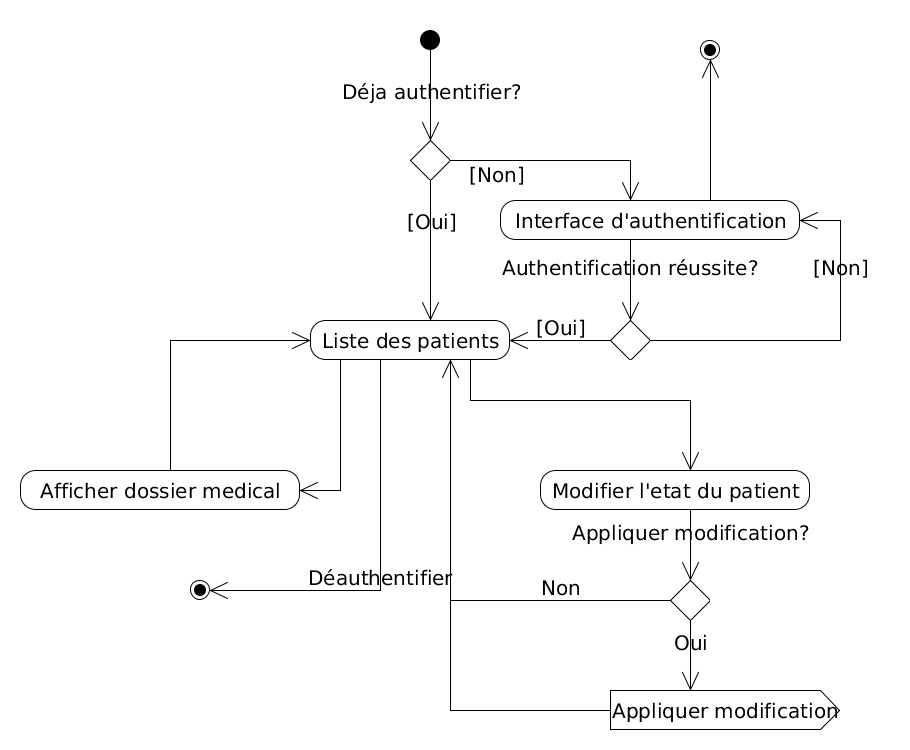
\includegraphics[width=0.8\textwidth]{diagrams/user_navigation}
\caption{Diagramme \gls{uml} d'activités de la navigation dans l'interface utilisateur.}
\label{fig:uml_act_ui}
\end{figure}

La figure \ref{fig:uml_act_ui} modélise par un diagramme \gls{uml} d'états le schéma que l'utilisateur suit pour naviguer dans l'interface utilisateur de notre application. Quelque Capture d'écran sont inclue pour illustrer le processus (figures \ref{fig:sc_login}, \ref{fig:sc_urgent}, \ref{fig:sc_display}, \ref{fig:sc_options}).

\begin{figure}
\center
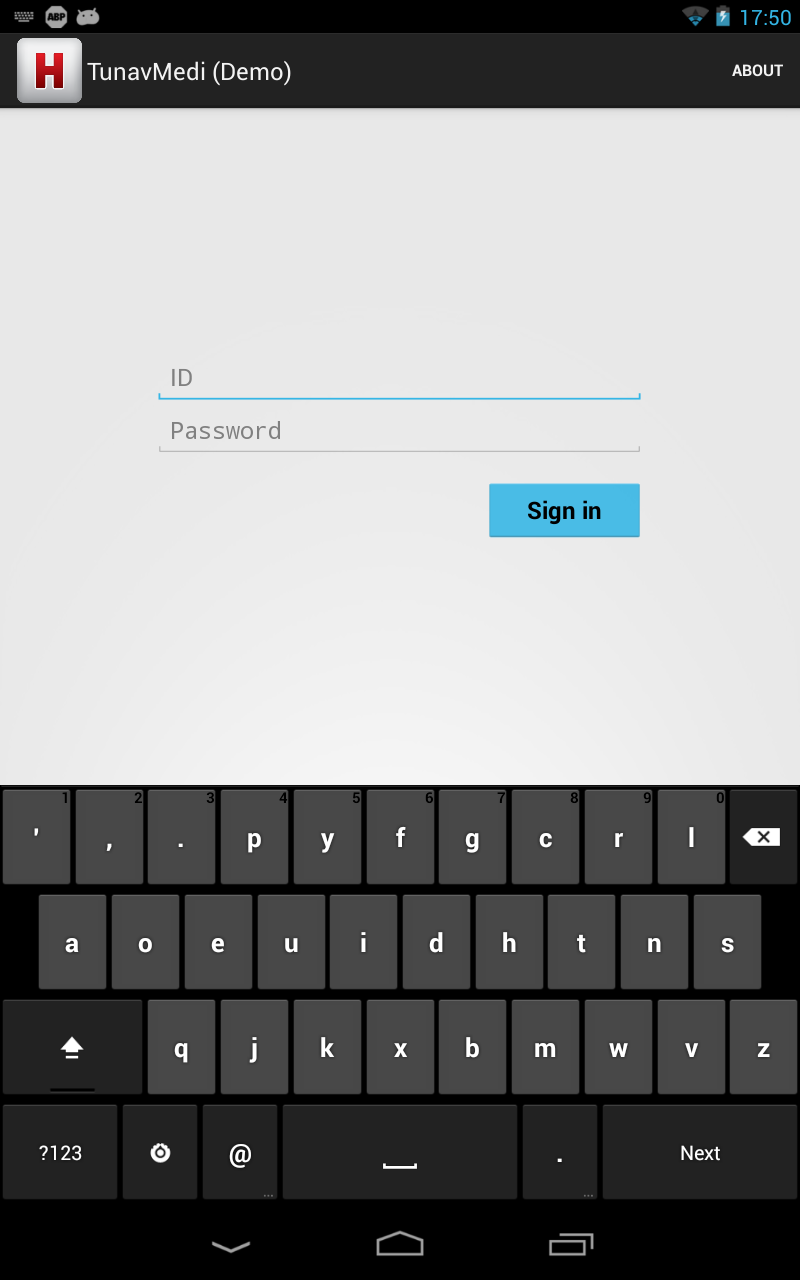
\includegraphics[height=0.4\textheight]{sc_login}
\caption{Interface graphique d'authentification.}
\label{fig:sc_login}
\end{figure}

\begin{figure}
\center
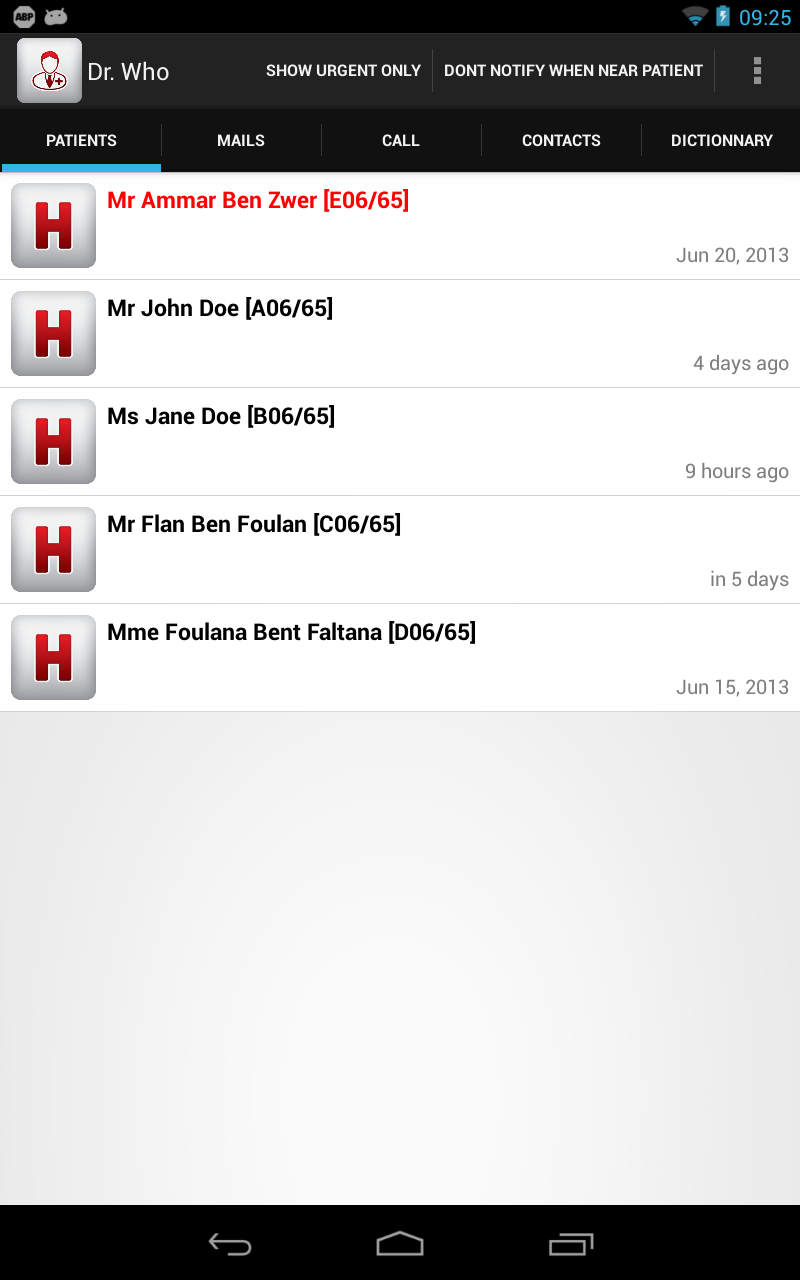
\includegraphics[height=0.4\textheight]{sc_urgent}
\caption{Capture écran de l'interface utilisateur de la liste des patients}
\label{fig:sc_urgent}
\end{figure}

\begin{figure}
\center
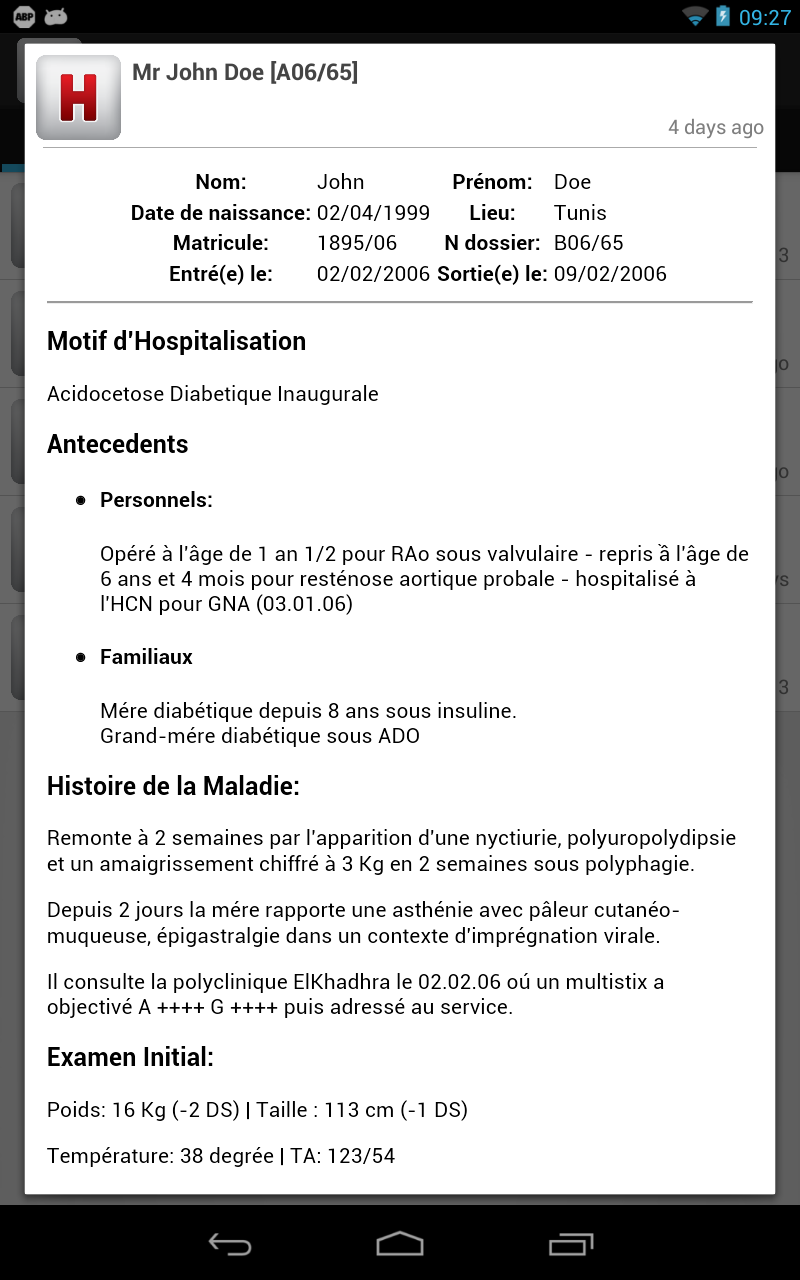
\includegraphics[height=0.4\textheight]{sc_display}
\caption{Capture écran de l'interface utilisateur relative à l'affichage du dossier médical du patient.}
\label{fig:sc_display}
\end{figure}

\begin{figure}
\center
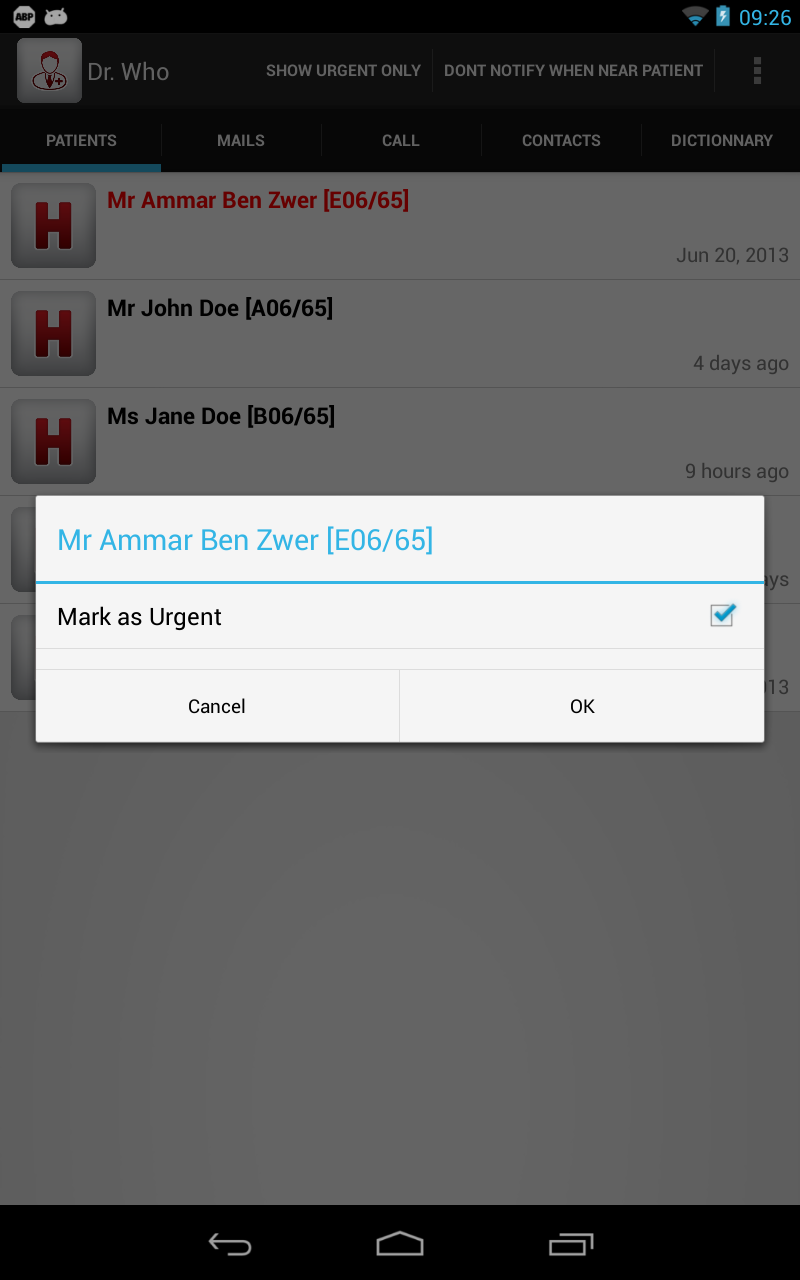
\includegraphics[height=0.4\textheight]{sc_options}
\caption{Capture écran de l'interface utilisateur affichée l'or de la modification de l’état du patient}
\label{fig:sc_options}
\end{figure}

\section{Authentification}

\begin{figure}
\center
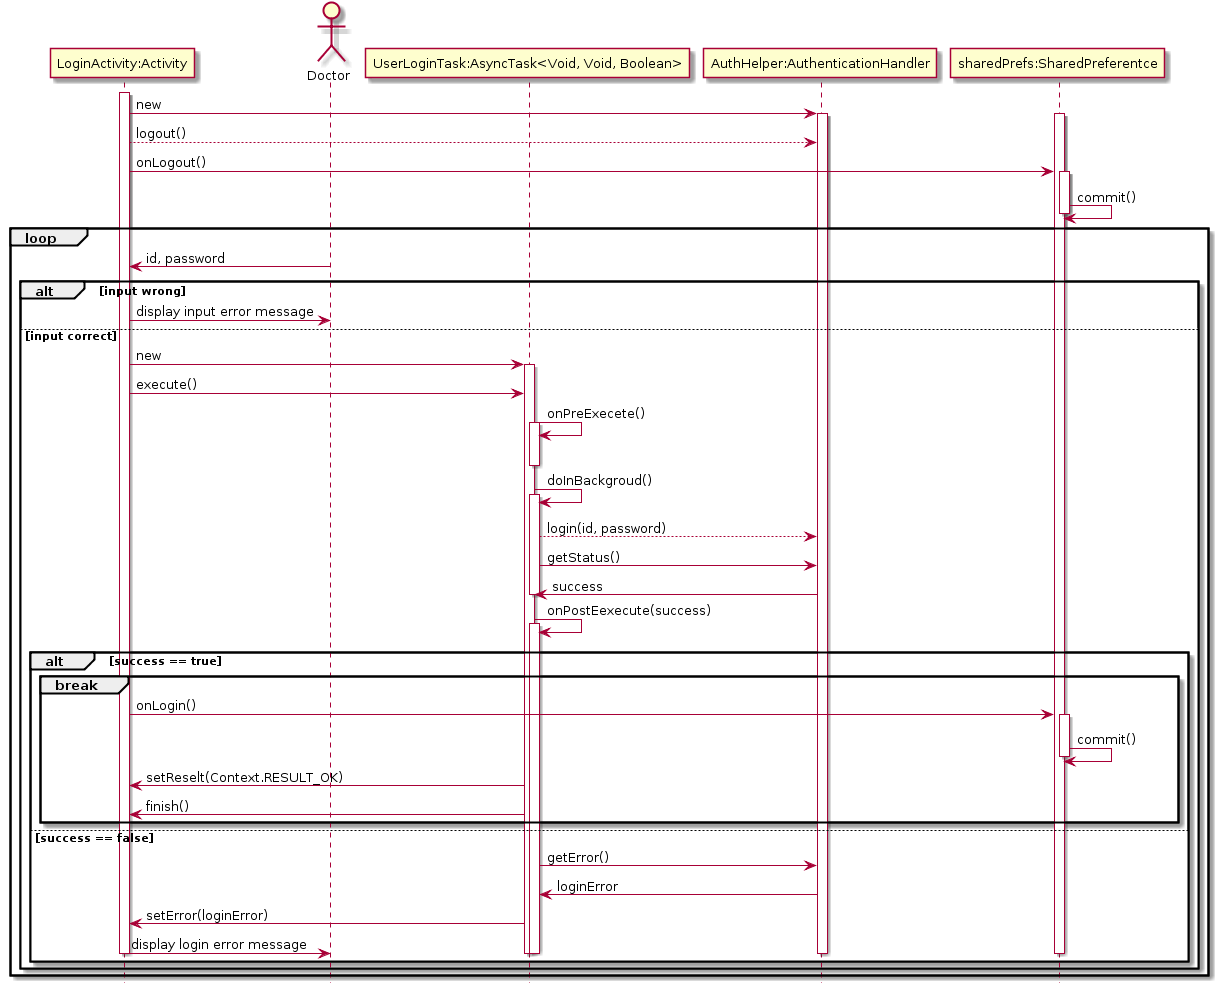
\includegraphics[angle=-90, width=\textwidth]{diagrams/seq_auth}
\caption{Diagramme \gls{uml} de séquence d'authentification.}
\label{fig:seq_auth}
\end{figure}

La figure \ref{fig:seq_auth} présente le comportement de l'application pour réaliser l'opération d'authentification de l'utilisateur à travers un diagramme de séquence \gls{uml}. On peut décrire textuellement le processus par les points suivants:

\begin{description}

\item[Acteurs:] Docteur.

\item[Pré-condition:] Le docteur est déjà inscrit dans la base de données du service et son identifiant et mot de passe lui sont fournit.

\item[Post-condition:] L'utilisateur est authentifier.

\item[Scénario nominal:]

\begin{enumerate}

\item L'utilisateur lance ou retourne à l'application mobile donc \dev{MainActivity}.

\item \dev{MainActivity} détecte que l'utilisateur n'est pas déjà authentifié et actionne l'\gls{ui} d'authentification (appel à \dev{LoginActivity}).

\item L'utilisateur saisit son identifiant et mot de passe.

\item L'application interpelle le service pour vérifier que la combinaison identifiant / mot de passe est correcte.

\item Le service distant retourne une réponse favorable, \dev{LoginActivity} enregistre les données relative à l'utilisateur.

\item \dev{LoginActivity} invoque \dev{MainActivity}.

\end{enumerate}

\item [Enchaînement alternatif:]

\begin{itemize}

\item 2.a L'utilisateur est déjà authentifier:

\begin{enumerate}

\item La séquence d'authentification est sautée.

\end{enumerate}

\item 3.a L’identifiant et / ou le mot de passe comporte des erreurs (champs vide, mot de passe comporte moins des caractères que le minimum):

\begin{enumerate}

\item Affichage d'un message d'erreur.

\end{enumerate}

\item 5.a Le service distant retourne une réponse défavorable:

\begin{enumerate}

\item Le message d'erreur est extrait de l'interface d'authentification.

\item \dev{LoginActivity} affiche le message d'erreur.

\end{enumerate}

\end{itemize}

\end{description}

\section{Afficher La Liste des Patients}
\section{Afficher Le dossier médical du patient}

\begin{figure}
\center
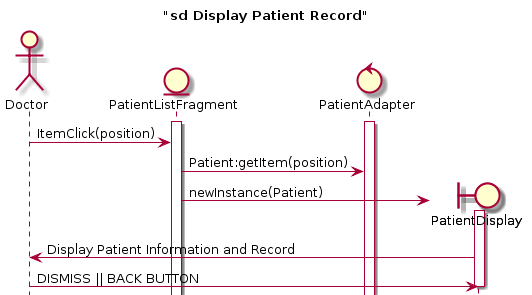
\includegraphics[width=0.8\textwidth]{diagrams/seq_display}
\caption{Diagramme de séquence \gls{uml} de l'affichage du dossier médical du patient.}
\label{fig:seq_display}
\end{figure}

La figure \ref{fig:seq_display} présente le comportement de l'application pour réaliser l'opération de l'affichage du dossier médical du patient à travers un diagramme de séquence \gls{uml}. On peut décrire textuellement le processus par les points suivants:

\begin{description}

\item[Acteurs:] Docteur.

\item[Pré-condition:] Le docteur s'est déjà authentifier et il se trouve sur l'interface de la liste des patients.

\item[Post-condition:] Le docteur à peut visualiser le dossier médical du patient qu'il à sélectionné.

\item[Scénario nominal:]

\begin{enumerate}

\item Le docteur clic sur un patient de la liste

\item \dev{PatientListFragment} détecte le clic et demande l'objet de type \dev{Patient} qui correspond au patient sélectionné par la méthode \dev{PatientAdapter.getItem()}.

\item L'objet \dev{Patient} reçu, \dev{PatientListFragment} crée une boite de  dialogue de type \dev{PatientDisplay} en lui passant l'objet Patient

\item \dev{PatientDisplay} affiche le dossier médical du patient.

\item Le docteur peut retourné à la liste des patient par un clic en dehors de la boite de dialogue ou par le bouton (retour).

\end{enumerate}

\end{description}

\section{Modification de l'Etat du patient}

\begin{figure}
\center
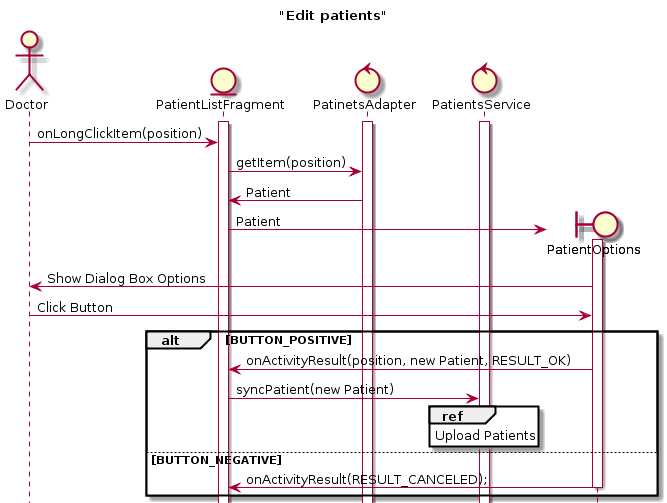
\includegraphics[width=0.8\textwidth]{diagrams/seq_editpatient}
\caption{Diagramme de séquence \gls{uml} de modification du status du patient}
\label{fig:seq_edit}
\end{figure}

La figure \ref{fig:seq_edit} présente le comportement de l'application pour réaliser l'opération de modification du status du patient (état normal ou état critique) à travers un diagramme de séquence \gls{uml}. On peut décrire textuellement le processus par les points suivants:

\begin{description}

\item[Acteurs:] Docteur.

\item[Pré-condition:] Le docteur s'est déjà authentifier et il se trouve sur l'interface de la liste des patients.

\item[Post-condition:] Le docteur à peut modifier le status du patient qu'il a sélectionné.

\item[Scénario nominal:]

\begin{enumerate}

\item Pour modifier le status d'un patient (cet patient est un cas urgent ou non) le médecin localise le patient dans la liste est fait un clic long sur son entrée.

\item Le \dev{PatientListFragment} détecte le clic long sur l'entrée du patient et demande au \dev{PatientAdapter} un objet patient à partir de sa position dans la liste à travers la méthode \dev{getItem()}.

\item L'objet \dev{Patient} correspondant au patient sélectionner reçu, le \dev{PatientListFragment} crée une boite de dialogue de type \dev{PatientOptions}.

\item La boite de dialogue \dev{PatientOptions} présente à l'utilisateur un checkbox avec deux boutons: bouton (OK) et bouton (Cancel) (figure \ref{fig:sc_options}).

\item Le médecin effectue le changement selon ses souhait et clic sur le bouton (OK).\label{item:alt}

\item \dev{PatientOptions} retourne à la \dev{PatientListFragment} l'objet Patient
mis à jour ainsi que sa position dans la liste et un drapeau
(RESULT\_OK).

\item La \dev{PatientListFragment} fait appel au \dev{PatientService} à travers sa méthode \dev{syncPatient()} et lui passe le patient modifier.

\item Le \dev{PatientService} effectue la séquence de mise à jour des patients (voir \ref{s:patientUpdate}).

\end{enumerate}

\item [Enchaînement alternatif:]

\begin{itemize}

\item \ref{item:alt}.a Le docteur clic sur le bouton (Cancel) au lieu du bouton (OK).
\begin{enumerate}

\item \dev{PatientOptions} retourne à la \dev{PatientListFragment} avec le drapeau (RESULT\_CANCELED).

\end{enumerate}

\end{itemize}


\end{description}

\section{Mise à jour des patients à partir du terminal}
\label{s:patientUpdate}

\section{Conclusion du Chapitre}
% %!TEX root = report.tex

\chapter{Déploiement et Tests}

\section{Introduction du Chapitre}

Ce chapitre porte sur les méthodes utilisées pour déployer notre application dans l'environnement de test ainsi que les techniques de teste utilisés.

\section{Déploiement}

Pour transférer notre application sur le terminal \android{} on utilise un outil fourni dans l'\gls{sdk}: \gls{adb}.

\gls{adb}\cite{tools:adb} est un outil versatile en ligne de commande qui nous permet de communiquer avec une instance d'un émulateur ou un équipement \android{} connecté. C'est un programme de type client-serveur qui inclue 3 composants:

\begin{itemize}

\item Un client, qui tourne sur notre machine de développement. On peut invoquer
un client depuis une invite de commande par l’envoi d'une commande \gls{adb}.
D'autre outils \android{} comme le plugin \gls{adt} et le \gls{ddms} crée eux
aussi des clients \gls{adb}.

\item Un serveur, qui tourne comme un processus de fond dans notre machine de
développement. Le serveur gère les communications entre le client et le démon
\gls{adb} qui tourne dans une instance d'un émulateur ou un terminal.

\item Un démon, qui tourne comme un processus de fond dans chaque instance de l’émulateur ou terminal.

\end{itemize}

On peut retrouver l'outil \gls{adb} dans le dossier $<sdk>/platform-tools/$.

On peut utiliser \gls{adb} pour copier une application depuis notre machine de développement et l'installer dans une instance d'un émulateur ou un terminal, pour cela on utilise la commande \cmd{install}. Cette commande exige comme paramètre le chemin du fichier .apk que nous voulons installer.


\begin{lstlisting}[language=bash, label=lst:adb_install, caption=Exemple d'utilisation du commande adb install]

$adb install ~/tunavmedi.apk

\end{lstlisting}

Notant qu'avec Eclipse équipé du plugin \gls{adt} on n'a pas besoin d'utiliser
\gls{adb} directement pour installer notre application sur l'émulateur ou le
terminal. Le plugin \gls{adt} s'occupe du packaging et de l'installation de
l'application pour nous.


Pour désinstaller une application on utilise le \en{Package Manager}. On peut
envoyer des commandes avec le \en{Package Manager} pour effectuer des actions et
des opérations de recherches sur les paquetages des applications installées dans
l'émulateur ou le terminal. Listing \ref{lst:adb_pm} présente la syntaxe
générale de l'outil tandis que le listing \ref{lst:adb_uninstall} présente la
syntaxe utilisé pour désinstaller notre application.


\begin{lstlisting}[language=bash, label=lst:adb_pm, caption=Syntaxe générale de l'utilisation du Package Manager]

$pm <command>

\end{lstlisting}

\begin{lstlisting}[language=bash, label=lst:adb_uninstall, caption=Exemple de désinstallation]

$adb shell pm uninstall com.tunav.tunavmedi

\end{lstlisting}

\subsection{Détecteur de bugs: Android Lint}

\begin{figure}[H]
\center
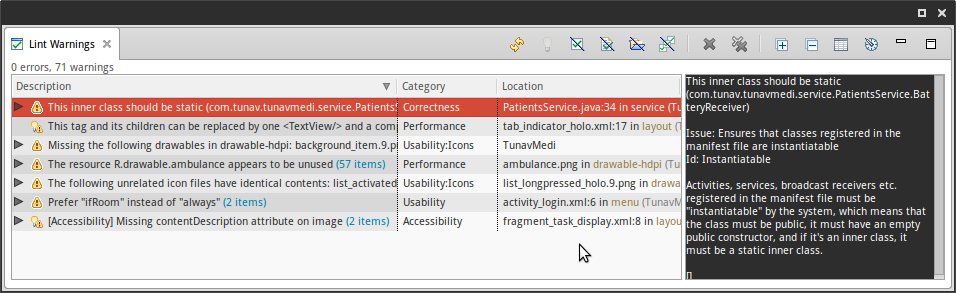
\includegraphics[width=0.9\textwidth]{lint}
\caption{Problèmes potentiels dans notre application détectés par Android Lint.}
\label{fig:lint}
\end{figure}

\android{} \en{Lint} (figure \ref{fig:lint}) est un outil introduit dans la version 16 de \gls{adt} qui scanne les code sources des projets \android{} afin d'y détecter des mal-fonctions potentielles.

Quelques exemples de types d'erreurs que cet outil permet de détecter sont:

\begin{itemize}

\item Translations manquantes ou inutilisés.

\item Les problèmes de performance dans les \dev{Layout}.

\item Ressources inutilisées

\item Tableau de taille inconsistante (dans le cas ou le tableau est défini dans des configurations différentes).

\item Problème d'accessibilités et d'internationalisation.

\item Problème d'icônes (Tailles manquantes, doubles, fausse résolution).

\item Problème d'usabilité .

\item Erreurs dans le \dev{Manifest}.

\end{itemize}

Dans Eclipse, \android{} Lint est disponible à travers le menu Window $\rightarrow$ Show View $\rightarrow$ Other... puis on sélectionne \en{Lint Warning} dans la fenêtre qui s'affiche (figure \ref{fig:lint_eclipse}).

\begin{figure}
\center
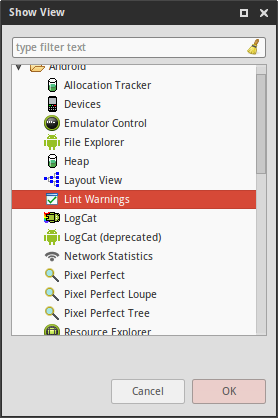
\includegraphics[width=0.4\textwidth]{lint_eclipse}
\caption{Accéder à Android Lint dans Eclipse}
\label{fig:lint_eclipse}
\end{figure}

\section[UI/Application Exerciser Monkey]{\en{UI/Application Exerciser Monkey}}

\en{Monkey} \cite{tools:monkey} est un programme qui tourne sur notre émulateur ou terminal \android{} et qui génère des flux pseudo-aléatoire d’événements utilisateur comme par exemple les clics, les touchés, les gestes, ou encore un nombre d’événements de niveau système. On peut utilisés \en{Monkey} pour effectuer des tests de stresse sur notre application dans une manière aléatoire et répétitive.

L'annexe \ref{chptr:monkey} montre un exemple de test effectué avec l'outil \en{Monkey} sur notre application.
%!TEX root = report.tex

\chapter*{Conclusion Générale}   
\addcontentsline{toc}{chapter}{Conclusion Générale}

L’intégration des technologies au sein des établissements médicaux est, malgré les divers obstacles, une tendance établie et représente un marché juteux pour les sociétés désirant le conquérir, et justifiant la judicieuse idée derrière ce projet.
Il en demeure que l’application en elle-même reste limitée. Et particulièrement, le processus de déploiement suggère un minimum d’infrastructures requises. Donc pour offrir l’expérience désirée, une solution alternative de support développée par TUNAV est de rigueur pour combler le manque dans les équipements de l’établissement  client ou, dans les cas extrêmes les supplanter. Une stratégie de commercialisation est un besoin évidant.
Ce projet peut être qualifié de type \og{}proof of concept\fg{}, il vise à explorer une idée et vérifier son applicabilité. Une aubaine pour l’application produite qui, en toute honnêteté, n’est pas encore au point et souffre de plusieurs lacunes de conceptions et d’implémentation. Si un produit sérieux dans le même thème est à offrir par TUNAV, des efforts de recherche et de développement sont de mise. En particulier l’intégration de médecins pratiquants dans des hôpitaux au processus de conception et de tests serait   critique pour la compétitivité du produit. 
Cependant, les problèmes techniques pour le développement de cette application ne sont pas les seuls à freiner son adoption. Outre le problème de coûts et l’effort de persuasion requis, c’est un problème d’ordre psychologique auquel il faut  faire face. En effet, avec tout concept qui change radicalement des procédures bien établies, une réticence de la part des utilisateurs ciblés, en l’occurrence les médecins, et le staff médical dans un contexte plus large, risque de saboter  les tests d´intégrations. Des campagnes  de sensibilisation sont à prévoir. 

%!TEX root = report.tex
\appendix

\chapter{UI/Application Exerciser Monkey}
\label{chptr:monkey}

\begin{lstlisting}[language=bash, label=lst:adb_monkey, caption=Utilisation de l'UI/Application Exerciser Monkey]

$ adb shell monkey -v -p com.tunav.tunavmedi 300
:Monkey: seed=1371512317847 count=300
:AllowPackage: com.tunav.tunavmedi
:IncludeCategory: android.intent.category.LAUNCHER
:IncludeCategory: android.intent.category.MONKEY
// Event percentages:
//   0: 15.0%
//   1: 10.0%
//   2: 2.0%
//   3: 15.0%
//   4: -0.0%
//   5: 25.0%
//   6: 15.0%
//   7: 2.0%
//   8: 2.0%
//   9: 1.0%
//   10: 13.0%
:Switch: #Intent;action=android.intent.action.MAIN;category=android.intent.category.LAUNCHER;launchFlags=0x10200000;component=com.tunav.tunavmedi/.activity.MainActivity;end
    // Allowing start of Intent { act=android.intent.action.MAIN cat=[android.intent.category.LAUNCHER] cmp=com.tunav.tunavmedi/.activity.MainActivity } in package com.tunav.tunavmedi
:Sending Touch (ACTION_DOWN): 0:(190.0,120.0)
:Sending Touch (ACTION_UP): 0:(191.60419,128.55092)
:Sending Trackball (ACTION_MOVE): 0:(3.0,-3.0)
:Sending Touch (ACTION_DOWN): 0:(473.0,23.0)
:Sending Touch (ACTION_UP): 0:(473.1426,23.805832)
:Sending Trackball (ACTION_MOVE): 0:(-5.0,3.0)
:Sending Trackball (ACTION_MOVE): 0:(3.0,0.0)
:Sending Trackball (ACTION_MOVE): 0:(-3.0,-5.0)
:Sending Touch (ACTION_DOWN): 0:(5.0,341.0)
:Sending Touch (ACTION_UP): 0:(4.349031,340.68045)
:Sending Trackball (ACTION_MOVE): 0:(2.0,-3.0)
:Sending Touch (ACTION_DOWN): 0:(611.0,766.0)
    //[calendar_time:2013-06-05 10:14:32.168  system_uptime:1098585565]
    // Sending event #100
:Sending Touch (ACTION_UP): 0:(678.4827,701.28955)
:Sending Touch (ACTION_DOWN): 0:(680.0,240.0)
:Sending Touch (ACTION_UP): 0:(669.64984,250.41994)
:Sending Trackball (ACTION_MOVE): 0:(1.0,2.0)
:Sending Trackball (ACTION_MOVE): 0:(-3.0,4.0)
:Sending Touch (ACTION_DOWN): 0:(33.0,339.0)
:Sending Touch (ACTION_UP): 0:(20.433603,303.77527)
:Sending Trackball (ACTION_MOVE): 0:(-4.0,-2.0)
:Sending Touch (ACTION_DOWN): 0:(556.0,636.0)
:Sending Touch (ACTION_UP): 0:(592.86835,561.529)
:Sending Trackball (ACTION_MOVE): 0:(2.0,2.0)
:Sending Touch (ACTION_DOWN): 0:(233.0,837.0)
:Sending Touch (ACTION_UP): 0:(226.95929,825.0325)
:Sending Touch (ACTION_DOWN): 0:(71.0,554.0)
:Sending Touch (ACTION_UP): 0:(73.91967,528.69226)
:Sending Touch (ACTION_DOWN): 0:(30.0,341.0)
:Sending Touch (ACTION_UP): 0:(84.22933,308.51373)
    //[calendar_time:2013-06-05 10:14:32.873  system_uptime:1098586237]
    // Sending event #200
    //[calendar_time:2013-06-05 10:14:32.874  system_uptime:1098586238]
    // Sending event #200
:Sending Trackball (ACTION_MOVE): 0:(1.0,-2.0)
:Sending Trackball (ACTION_MOVE): 0:(-3.0,0.0)
:Sending Trackball (ACTION_UP): 0:(0.0,0.0)
:Sending Touch (ACTION_DOWN): 0:(782.0,261.0)
:Sending Touch (ACTION_UP): 0:(789.2555,259.95465)
:Sending Touch (ACTION_DOWN): 0:(480.0,1180.0)
:Sending Touch (ACTION_UP): 0:(517.4512,1113.8969)
:Sending Touch (ACTION_DOWN): 0:(775.0,965.0)
:Sending Touch (ACTION_UP): 0:(762.51733,968.3565)
:Sending Trackball (ACTION_MOVE): 0:(4.0,-4.0)
:Sending Trackball (ACTION_MOVE): 0:(1.0,-2.0)
:Sending Trackball (ACTION_MOVE): 0:(-3.0,1.0)
:Sending Touch (ACTION_DOWN): 0:(89.0,1185.0)
:Sending Touch (ACTION_UP): 0:(109.65848,1195.4576)
:Sending Trackball (ACTION_MOVE): 0:(-4.0,-5.0)
:Sending Touch (ACTION_DOWN): 0:(339.0,280.0)
:Sending Touch (ACTION_UP): 0:(351.69287,274.5476)
:Sending Trackball (ACTION_MOVE): 0:(0.0,-1.0)
Events injected: 300
:Sending rotation degree=0, persist=false
:Dropped: keys=0 pointers=0 trackballs=0 flips=0 rotations=0
## Network stats: elapsed time=1986ms (0ms mobile, 1986ms wifi, 0ms not connected)

\end{lstlisting}

\chapter{Logiciel de gestion de versions Git}

\begin{figure}
\center

\includegraphics[width=0.4\textwidth]{git_logo}
\caption{Logo du logiciel de gestion de version Git}
\label{fig:git}
\end{figure}

\en{Git}\cite{wikipedia:git} est un système de gestion de versions et un gestionnaire de code source connu pour sa rapidité. Conçu et développée initialement par \textsf{Linus Torvalds} pour le développement du \en{Kernel} \en{Linux}, Git a depuis éte adopter par plusieurs autre projets.

Chaque répertoire de travail de Git est un dépôt complet avec un historique complet et des capacité de suivit de version, il est indépendant d'un accès réseau ou d'un serveur centrale.

Git est un logiciel libre distribuer sous les termes de la licence  \en{GNU General Public License} version 2.

L'usage de Git est très simple, un des workflow simplifier serai comme suit:

\begin{itemize}

\item La branche master contient la dernière version de l'application. Malheureusement, cette version contient un bug dans le \dev{MenuItem}

\item Pour éviter, pendant qu'on corrige le bug, d'altérer la version courante de  l'application de façon nuisible, on crée une branche différente ou on peut tester nos modification tranquillement (listing \ref{lst:git_branch}).

\item On peut passer vers la nouvelle branche crée précédemment (listing \ref{lst:git_checkout}).

\item On à maintenant réussi a corrigé le bug en question, et aussi travailler un peut sur notre rapport. On peut avoir un rapport sur les fichiers modifier pendant ce processus (listing \ref{lst:git_status}).

\item Après on peut appliquer nos changements dans la branche master de notre répertoire Git (listing \ref{lst:git_merge}).

\end{itemize}

\begin{lstlisting}[language=bash, label=lst:git_branch, caption=Git Branch]

\end{lstlisting}

\begin{lstlisting}[language=bash, label=lst:git_checkout, caption=Git checkout]

\end{lstlisting}

\begin{lstlisting}[language=bash, label=lst:git_status, caption=Git status]

➜  PFE git:(bug_MenuItem) ✗ git status

# On branch bug_MenuItem
# Changes not staged for commit:
#   (use "git add <file>..." to update what will be committed)
#   (use "git checkout -- <file>..." to discard changes in working directory)
#
#   modified:   README.md
#   modified:   pfe.sublime-project
#   modified:   report/2_cadre_general.tex
#   modified:   report/4_travail.tex
#   modified:   report/acronyms.tex
#   modified:   report/appendix.tex
#   modified:   report/bibliography.bib
#   modified:   report/report.pdf
#   modified:   report/report.tex
#   modified:   res/ep/Scenarios.ep
#   modified:   res/ep/architecture.ep
#   modified:   source/tunavmedi/src/com/tunav/tunavmedi/fragment/PatientListFragment.java
#
# Untracked files:
#   (use "git add <file>..." to include in what will be committed)
#
#   res/architecture-interfaces.png
#   res/ep/scenarioactors.png
#   res/ep/scenarioalltunav.png
#   res/ep/scenariointeractions.png
#   res/ep/scenarioother.png
#   res/sc_display.png
#   res/sc_options.png
#   res/sc_urgent.png
no changes added to commit (use "git add" and/or "git commit -a")

\end{lstlisting}

\begin{lstlisting}[language=bash, label=lst:git_merge, caption=Git merge]

\end{lstlisting}

\bibliography{bibliography}
\label{LastPage}

\end{document}
